\documentclass[conference]{IEEEtran}
\IEEEoverridecommandlockouts

\usepackage{cite}
\usepackage{amsmath,amssymb,amsfonts}
\usepackage{algorithmic}
\usepackage{graphicx}
\graphicspath{{figuras/}}
\usepackage{textcomp}
\usepackage{xcolor}
\usepackage{booktabs}
\usepackage{multirow}
\usepackage{array}
\usepackage{siunitx}
\usepackage[hidelinks]{hyperref}
\usepackage{float}
\usepackage{caption}
\usepackage{placeins}

\def\BibTeX{{\rm B\kern-.05em{\sc i\kern-.025em b}\kern-.08em
    T\kern-.1667em\lower.7ex\hbox{E}\kern-.125emX}}

% ---------- placeholder helpers ----------
\newcommand{\PH}[1]{\fbox{\parbox{0.92\linewidth}{\footnotesize\itshape #1}}}
\newcommand{\IMG}[2]{%
  \begin{figure}[H]
    \centering
    \fbox{\parbox{0.9\linewidth}{\centering\vspace{2.2cm}\itshape\footnotesize #1\vspace{2.2cm}}}
    \caption{#2}
  \end{figure}
}

% Fotografía del montaje a ancho de columna, sin el recuadro de los marcadores de posición.
\newcommand{\FOTO}[2]{%
  \begin{figure}[H]
    \centering
    \includegraphics[width=\linewidth]{#1}
    \caption{#2}
  \end{figure}
}

% Imagen a página completa (para el índice de cálculos a mano en el Apéndice).
% Uso: \IMGPAGE{texto del placeholder o ruta con \includegraphics}{pie de figura}
\newcommand{\IMGPAGE}[2]{%
  \clearpage
  \begin{figure*}[p]
    \centering
    \fbox{\parbox[c][0.85\textheight][c]{0.96\linewidth}{\centering\itshape #1}}
    \caption{#2}
  \end{figure*}
  \clearpage
}

\begin{document}

\title{Diseño e Implementación de un Controlador PID Analógico con Amplificadores Operacionales para un Sistema de Levitación Electromagnética}

\author{
\IEEEauthorblockN{Brahiam Alberto Campiño Romero}
\IEEEauthorblockA{\textit{Programa de Ingeniería Electrónica} \\
\textit{Universidad de Ibagué}\\
Ibagué-Tolima, Colombia \\
brahiam.campino@estudiantesunibague.edu.co}
}

\maketitle

\begin{abstract}
Se presenta el diseño, el cálculo teórico y la implementación de un controlador Proporcional-Integral-Derivativo (PID) completamente analógico, construido con amplificadores operacionales, destinado a estabilizar la posición de un objeto en levitación mediante fuerza electromagnética de atracción. El controlador entrega una señal de salida que varía entre 1~V y 3~V, proporcional al estado de corrección requerido por el sistema. Se justifica la elección del PID frente a alternativas de control más simples, se derivan las ecuaciones de diseño de cada etapa (diferenciador de error, proporcional, integral con anti-windup, derivativo y sumador), y se documentan las correcciones realizadas durante la etapa experimental, entre ellas la saturación del integrador y del sumador, y el efecto de carga observado en los divisores resistivos utilizados para generar los voltajes de referencia y de offset. Los resultados teóricos se contrastan con las mediciones obtenidas sobre el circuito implementado.
\end{abstract}

\begin{IEEEkeywords}
control PID analógico, amplificador operacional, levitación magnética, anti-windup, control de posición, LM741
\end{IEEEkeywords}

% =========================================================
\section{Introducción y Justificación del Controlador}
% =========================================================

Un sistema de levitación electromagnética por atracción es, por naturaleza, un sistema inestable en lazo abierto: la fuerza de atracción entre el electroimán y el objeto aumenta al disminuir la distancia entre ambos, de modo que cualquier desviación respecto al punto de equilibrio tiende a crecer en lugar de corregirse por sí sola. Este comportamiento está respaldado por el teorema de Earnshaw~\cite{earnshaw1842}, que demuestra que ninguna configuración estática de imanes puede sostener un cuerpo en equilibrio estable sin control activo.

Antes de seleccionar la estrategia de control se evaluaron las siguientes alternativas:

\begin{itemize}
\item \textbf{Control todo-o-nada:} produce una fuerza discontinua, generando oscilaciones bruscas incompatibles con un posicionamiento fino y continuo.
\item \textbf{Proporcional (P) puro:} reacciona de forma instantánea al error, pero al no tener memoria del pasado, su salida es nula en el punto de equilibrio exacto (error nulo), dejando un error de estado estable permanente.
\item \textbf{Proporcional-Derivativo (PD):} añade amortiguamiento y mejora la estabilidad dinámica, pero conserva el error de estado estable al carecer de acción integral.
\item \textbf{Proporcional-Integral-Derivativo (PID):} combina los tres efectos de forma paralela. El término proporcional corrige el error instantáneo, el integral elimina el error de estado estable acumulando el historial reciente del error, y el derivativo introduce el amortiguamiento que el sistema no posee de forma natural, al no existir fricción mecánica real en un sistema sin contacto.
\end{itemize}

Matemáticamente, el controlador PID se expresa como la suma de tres términos independientes:
\begin{equation}
u(t) = K_p\,e(t) + K_i\int_0^t e(\tau)\,d\tau + K_d\,\frac{de(t)}{dt}
\label{eq:pid}
\end{equation}

Es fundamental resaltar que los tres términos se implementan en configuración \emph{paralela} y no en cascada: la definición matemática del PID es una suma, y una conexión en serie alteraría la función de transferencia resultante, acoplando las ganancias $K_p$, $K_i$ y $K_d$ entre sí e impidiendo su ajuste independiente.

% =========================================================
\section{Marco Teórico de Cada Etapa}
% =========================================================

La nomenclatura de referencia utilizada en esta sección corresponde a la Tabla~\ref{tab:nomenclatura}.

\subsection{Amplificador diferenciador de error}
Compara el voltaje del sensor de posición ($V_{sensor}$) contra el voltaje de referencia ($V_{ref}$). Con $R_1=R_3$ y $R_{2}=R_4$:
\begin{equation}
V_e = \frac{R_{2}}{R_1}\left(V_{ref}-V_{sensor}\right)
\label{eq:diff}
\end{equation}
$V_e$ alimenta en paralelo a las ramas P, I y D.

\subsection{Etapa Proporcional (P)}
Amplificador inversor simple, sin memoria:
\begin{equation}
V_P(t) = -K_p\,V_e(t) = -\frac{Pot_{1}}{R_5}\,V_e(t)
\label{eq:p}
\end{equation}
Por sí sola deja un error de estado estable, pues su salida es nula cuando el error es nulo.

\subsection{Etapa Integral (I)}
Acumula el historial del error, eliminando el error de estado estable que deja P:
\begin{equation}
V_I(t) = -\frac{1}{R_i C_i}\int V_e(t)\,dt
\label{eq:i}
\end{equation}
Un integrador ideal posee memoria infinita, lo que provoca saturación (\emph{windup}) ante cualquier offset residual del amplificador operacional. Se incorpora una resistencia de fuga $R_6$ en paralelo con $C_i$, acotando la ganancia en continua a un valor finito y dotando al integrador de una memoria efectiva finita $\tau = R_6 C_i$:
\begin{equation}
G_{DC,max} = \frac{R_{11}}{Pot_2}, \qquad f_{aw} = \frac{1}{2\pi R_{11} C_i}
\label{eq:i_aw}
\end{equation}

\subsection{Etapa Derivativa (D)}
Responde a la velocidad de cambio del error, aportando el amortiguamiento que el sistema no posee de forma natural:
\begin{equation}
V_D(t) = -Pot_{3}\,C_2\,\frac{dV_e(t)}{dt}
\label{eq:d}
\end{equation}
Se agrega una resistencia $R_7$ en serie con $C_2$ para limitar la ganancia a alta frecuencia y no amplificar ruido:
\begin{equation}
G_{max} = \frac{Pot_{3}}{R_6}, \qquad f_c = \frac{1}{2\pi R_6 C_2}
\label{eq:d_fc}
\end{equation}
Esta etapa opera normalmente en el rango de milivoltios y no de voltios, ya que su salida depende de qué tan rápido cambia el error ($de/dt$) y no de su magnitud. Dado que la posición del objeto varía de forma mecánica —relativamente lenta frente a la respuesta eléctrica del circuito— $de/dt$ es pequeña la mayor parte del tiempo, y $V_D$ solo alcanza el rango de voltios durante una perturbación brusca. El voltaje residual de pocos milivoltios observado en reposo corresponde principalmente al offset de entrada propio del amplificador operacional (1 a 6~mV típico en el LM741), no a una derivada real distinta de cero.

\subsection{Etapa Sumadora}
Combina $V_P$, $V_I$, $V_D$ y el offset $V_{off}$:
\begin{equation}
V_{PID} = -\left(\frac{R_{10}}{R_7}V_P+\frac{R_{10}}{R_8}V_I+\frac{R_{10}}{R_{9}}V_D+\frac{R_{10}}{R_{offset}}V_{off}\right)
\label{eq:sum}
\end{equation}
Es la salida final del controlador, con rango de operación objetivo entre 1~V y 3~V.

\subsection{Generación de \texorpdfstring{$V_{ref}$}{Vref} y \texorpdfstring{$V_{off}$}{Voff}}
Para evitar fuentes adicionales, $V_{ref}$ y $V_{off}$ se generan desde una única fuente mediante divisores resistivos. Un divisor cargado por la etapa siguiente entrega un voltaje distinto al calculado (efecto de carga); por ello cada divisor se desacopla con un amplificador operacional en configuración de seguidor de voltaje (buffer no inversor, ganancia unitaria), de alta impedancia de entrada y baja impedancia de salida, que preserva el voltaje calculado sin alterarlo.

% =========================================================
\section{Cálculos de Diseño}
% =========================================================

Esta sección presenta la derivación completa de cada etapa a partir del análisis nodal del amplificador operacional (corriente de entrada nula, corto virtual entre sus terminales).

\subsection{Diferenciador de error}
Con $R_1=R_3$, $R_2=R_4$, corto virtual ($V^-=V^+$) y $I_1=I_2$:
\begin{align}
I_1 &= \frac{V_1-V^+}{R_1} = I_2 = \frac{V^+-V_{out}}{R_2} \\
-\frac{V_{out}}{R_2} &= \frac{V_1}{R_1}-V^+\left(\frac{1}{R_1}+\frac{1}{R_2}\right) \\
V_{out} &= \left(1+\frac{R_2}{R_1}\right)V^+ - V_1\frac{R_2}{R_1}
\end{align}
Sustituyendo el divisor de la rama no inversora, $V^+=V_2\dfrac{R_2}{R_1+R_2}$, y simplificando:
\begin{equation}
\boxed{V_{out}=\frac{R_2}{R_1}\left(V_1-V_2\right)=\frac{R_2}{R_1}\,V_s}, \qquad A_v=\frac{R_2}{R_1}
\label{eq:diff_full}
\end{equation}

\textbf{Diseño:} se propone una ganancia unitaria para obtener la diferencia sin alterar las magnitudes de entrada:
\begin{equation}
A_v=1,\qquad R_1=10\,\text{k}\Omega,\qquad V_{CC}>V_{out},\qquad V_{ref}=2\,\text{V}
\end{equation}
\textbf{Condiciones de voltajes máximos, medios y mínimos:}
\begin{equation}
V_{out,max}=(5\text{V}-2\text{V})=\boxed{3\,\text{V}}
\end{equation}
\begin{equation}
V_{out,min}=(0\text{V}-2\text{V})=\boxed{-2\,\text{V}}
\end{equation}
\begin{equation}
V_{out,mid}=(2\text{V}-2\text{V})=\boxed{0\,\text{V}}
\end{equation}
\textbf{Despeje de $R_2$:}
\begin{equation}
R_2=A_v\cdot R_1
\end{equation}
Con $V_{CC,general}=16\,\text{V}$, los valores finales de diseño son:
\begin{equation}
A_v=1,\quad R_1=10\,\text{k}\Omega,\quad R_2=10\,\text{k}\Omega,\quad V_{CC}=\pm16\,\text{V}
\end{equation}
\textbf{Ecuación final:}
\begin{equation}
V_{out}=\left(V_{sensor}-V_{ref}\right)
\end{equation}

\subsection{Etapa Proporcional (P)}
Con $V^-=0$ (entrada no inversora a tierra) e $I_1=I_2$:
\begin{equation}
\frac{V_{out1}}{R_5}=-\frac{V_{out2}}{Pot_1} \;\Rightarrow\; \boxed{A_v=\frac{Pot_1}{R_5}}
\label{eq:p_full}
\end{equation}
\textbf{Diseño:} con $R_5=10\,\text{k}\Omega$ y $V_{out,max}=3\,\text{V}$ como referencia de prueba:
\begin{equation}
Pot_1 = K_p\cdot R_5
\end{equation}
Valores evaluados: $K_p=1\Rightarrow Pot_1=10\,\text{k}\Omega$; $K_p=2\Rightarrow Pot_1=20\,\text{k}\Omega$. El potenciómetro se dispuso para variar de $10\,\text{k}\Omega$ a $20\,\text{k}\Omega$ según el punto de ajuste deseado.

\subsection{Etapa Integral (I)}
\textbf{Elección de $f_{aw}$:} se parte de la dinámica reportada en la literatura de referencia (oscilaciones entre 2 y 5~Hz~\cite{berkelman}), ubicando $f_{aw}$ con margen amplio por debajo de dicho rango:
\begin{equation}
f_{aw}=0.2\,\text{Hz}, \qquad C_i = 1\,\mu\text{F}
\end{equation}
\begin{equation}
R_{11}=\frac{1}{2\pi\,(0.2)(1\mu F)}\approx 800\,\text{k}\Omega
\end{equation}
\textbf{Constante de integración:}
\begin{equation}
K_i=\frac{1}{R_i C_i}=10\,\text{s}^{-1} \;\Rightarrow\; Pot_2=\frac{1}{(1\mu F)(10)}=10\,\text{k}\Omega
\end{equation}
\textbf{Derivación por Laplace (integrador ideal), condiciones iniciales nulas:}
\begin{equation}
V_{out}(s)=-\frac{1}{Pot_2\,C_i}\cdot\frac{V_e(s)}{s}, \qquad H(s)=-\frac{1}{Pot_2\,C_i\,s}
\end{equation}
Sustituyendo $s=j2\pi f$ y tomando magnitud:
\begin{equation}
\boxed{|H(j\omega)|=\frac{1}{2\pi\,Pot_2\,f\,C_i}}
\end{equation}
\textbf{Integrador con fuga} ($R_6 \parallel C_i$, topología correcta tras la corrección descrita en la Sección~\ref{sec:ajustes}):
\begin{equation}
Z_f(s)=R_{11}\parallel\frac{1}{sC_i}=\frac{R_{11}}{1+sR_{11}C_i}
\end{equation}
\begin{equation}
|H(j\omega)|=\frac{R_{11}/Pot_2}{\sqrt{1+(f/f_{aw})^2}}
\end{equation}
Evaluando en $f=0$ se obtiene la ganancia máxima en continua:
\begin{equation}
K_{i,max}=\left.\frac{R_{11}/Pot_2}{\sqrt{1+0}}\right. = \frac{R_{11}}{Pot_2}=\frac{1\text{M}}{12.5\text{k}}=\boxed{80}
\end{equation}

\subsection{Etapa Derivativa (D)}
\textbf{Limitación de ganancia en alta frecuencia:} dado que $Z_C=1/(2\pi f C)\to 0$ a alta frecuencia, un diferenciador puro amplificaría el ruido sin límite. $R_7$ fija un piso mínimo de impedancia:
\begin{equation}
R_7 \le \frac{1}{2\pi f_c C_2}
\end{equation}
\textbf{Elección de $f_d$} (frecuencia de corte, término medio entre la dinámica del sistema y el ruido de alta frecuencia, valor de prueba):
\begin{equation}
f_d = 150\,\text{Hz}, \qquad C_2 = 1\,\mu\text{F}
\end{equation}
\begin{equation}
R_7=\frac{1}{2\pi(150)(1\mu F)}=1.06\,\text{k}\Omega\approx\boxed{1\,\text{k}\Omega}
\end{equation}
\textbf{Ganancia:}
\begin{equation}
K_d=\frac{Pot_3}{R_6}
\end{equation}
Con $K_d=21$ como punto de diseño:
\begin{equation}
Pot_3=K_d\cdot R_6 = 21\times1\text{k}=21\,\text{k}\Omega\approx\boxed{22\,\text{k}\Omega} \;(K_{d,max}=22)
\end{equation}

\subsection{Etapa Sumadora}
Condiciones de partida (op-amp ideal): $I_{in}=0$, corto virtual entre terminales. Criterio de diseño: se busca ganancia unitaria por rama para no alterar los valores de $K_p$, $K_i$ y $K_d$ ya calculados; las resistencias no deben ser demasiado altas (acoplan ruido) ni demasiado bajas (cargan la salida del operacional anterior).

Con $R_8=R_9=R_{10}=R_{7}\,\text{k}\Omega$ (entradas y realimentación iguales, $A_{vs}=1$), el análisis nodal en el nodo inversor ($V^-$, corto virtual con $V^+=0$), incluyendo la rama de offset, da:
\begin{equation}
\frac{V^--0}{R_{eq}}=\frac{0-V_{out}}{R_{10}}
\end{equation}
\begin{equation}
-\frac{V_P}{R_7}-\frac{V_I}{R_8}-\frac{V_D}{R_{9}}=-\frac{V_{out}}{R_{10}}
\end{equation}
Con ganancia unitaria por rama ($R_{10}=R_8=R_9=R_{7}=R_{offset}$):
\begin{equation}
V_{out}=R_{10}\left(\frac{V_P}{R_{10}}+\frac{V_I}{R_{10}}+\frac{V_D}{R_{10}}\right)
\end{equation}
\begin{equation}
\boxed{V_{out}=V_P+V_I+V_D}
\end{equation}
\textbf{Resistencia de compensación de bias} en la entrada no inversora:
\begin{equation}
R_{bias}=R_8\parallel R_9\parallel R_{7} = 10\text{k}\parallel10\text{k}\parallel10\text{k}=
\boxed{3.3\,\text{k}\Omega}
\end{equation}

\subsection{Divisores de \texorpdfstring{$V_{off}$}{Voff} y \texorpdfstring{$V_{ref}$}{Vref}}
\textbf{Divisor de $V_{off}$} ($V_{CC}=16\,$V, $R_{15}=160\,\text{k}\Omega$ fijo, objetivo $V_{out}=10\,$V antes del buffer):
\begin{equation}
V_{out}=V_{CC}\cdot\frac{R_{15}}{R_{15}+R_{14}} \;\Rightarrow\; R_{14}=\frac{V_{CC}\,R_{15}}{V_{out}}-R_{15}
\end{equation}
\begin{equation}
R_{14}=\frac{(16)(160\text{k})}{10}-160\text{k}=\boxed{96\,\text{k}\Omega}
\end{equation}
\textbf{Divisor de $V_{ref}$} ($R_{13}=160\,\text{k}\Omega$ fijo, objetivo $V_{out}=2\,$V):
\begin{equation}
R_{12}=\frac{V_{CC}\,R_{13}}{V_{out}}-R_{13}
\end{equation}
\begin{equation}
R_{12}=\frac{(16)(160\text{k})}{2}-160\text{k}=\boxed{1.12\,\text{M}\Omega}
\end{equation}
\PH{Nota de verificación: en el desarrollo a mano de esta etapa se registró $V_{CC}=5\,$V para el divisor de $V_{ref}$, lo que da $R_{12}=\frac{(5)(160\text{k})}{2}-160\text{k}=240\,\text{k}\Omega$. Confirmar con el montaje físico cuál de las dos fuentes (5~V dedicada o 16~V compartida) alimenta realmente esta rama antes de fijar el valor definitivo de $R_{12}$.}

% =========================================================
\section{Ajustes Realizados Durante las Pruebas}
\label{sec:ajustes}
% =========================================================

\subsection{Saturación de la etapa sumadora}
Al evaluar la salida del controlador con un error cercano al máximo esperado, se observó que la salida del sumador tendía a saturarse contra los rieles de alimentación por su alta ganancia (la cual era de 23.24v) cuando su alimentación max es de 18v. Para solucionarlo se bajo la ganancia unitaria del sumador por una de 0.1 veces en todas las ramas para no afectar a los datos de control, además se bajo la ganancia propuesta anteriormente de P para acercarse mas a los valores requeridos.

\textbf{Ajuste del rango de salida (1~V a 3~V):} con las ganancias iniciales de diseño, se evalúa el error mínimo y máximo del sistema:
\begin{equation}
V_{error,min}=0+0+0\approx 0\,\text{V}
\end{equation}
\begin{equation}
V_{error,max}=9.90+13.5+3.24\times10^{-3}=23.24\,\text{V} \quad(\text{excesivo})
\end{equation}
Se corrige bajando la ganancia del sumador de 1 a 0.1 (resistencia de realimentación $R_{12}$ de $10\,\text{k}\Omega$ a $1\,\text{k}\Omega$):
\begin{equation}
\begin{aligned}
V_{out,max}&=\tfrac{1\text{k}}{10\text{k}}(9.9)+\tfrac{1\text{k}}{10\text{k}}(13.3)\\
&+\tfrac{1\text{k}}{10\text{k}}(3\times10^{-3})+\tfrac{1}{10\text{k}}(10)=3.34\,\text{V}
\end{aligned}
\end{equation}
Se agrega el voltaje de offset para fijar el piso en 1~V:
\begin{equation}
\begin{aligned}
V_{out,min}&=\tfrac{1\text{k}}{10\text{k}}(0)+\tfrac{1\text{k}}{10\text{k}}(0)\\
&+\tfrac{1\text{k}}{10\text{k}}(0)+\tfrac{1}{10\text{k}}(10)=\boxed{1\,\text{V}}
\end{aligned}
\end{equation}
Finalmente se reduce $K_p$ de 3 a $K_p=2.2$ ($Pot_1=22\,\text{k}\Omega$) para que el valor máximo converja exactamente a 3~V:
\begin{equation}
\begin{aligned}
V_{out,max}&=\tfrac{1\text{k}}{10\text{k}}(6.6)+\tfrac{1\text{k}}{10\text{k}}(13.3)\\
&+\tfrac{1\text{k}}{10\text{k}}(3\times10^{-3})+\tfrac{1}{10\text{k}}(10)=\boxed{3.02\,\text{V}}
\end{aligned}
\end{equation}
Ecuacion del sumador modificada.
\begin{equation}
-\frac{V_P}{R_7}-\frac{V_I}{R_8}-\frac{V_D}{R_{9}}-\frac{V_{off}}{R_{offset}}=-\frac{V_{out}}{R_{10}}
\end{equation}
Con ganancia unitaria por rama ($R_{10}=R_8=R_9=R_{7}=R_{offset}$):
\begin{equation}
V_{out}=R_{10}\left(\frac{V_P}{R_{10}}+\frac{V_I}{R_{10}}+\frac{V_D}{R_{10}}+\frac{V_{off}}{R_{10}}\right)
\end{equation}

Nueva Rbias.
\begin{equation}
R_{bias}=R_8\parallel R_9\parallel R_{7}\parallel R_{offset} = 10\text{k}\parallel10\text{k}\parallel10\text{k}\parallel10\text{k}=
\boxed{4.4\,\text{k}\Omega}
\end{equation}

\subsection{Saturación y corrección de topología de la etapa integral}
En una primera implementación, la resistencia de anti-windup se conectó \emph{en serie} con el capacitor de integración, en lugar de en paralelo. Esta configuración deja la rama de realimentación en circuito abierto en corriente continua (el capacitor en serie bloquea el paso de DC), dejando al amplificador operacional sin una realimentación negativa bien definida en ese régimen y produciendo un comportamiento dominado por el desbalance interno del propio amplificador, en lugar de la función de integración esperada. Al corregir la conexión a su posición correcta ($R_{11} \parallel C_i$), el circuito recuperó el comportamiento esperado: salida nula para error nulo y respuesta en rampa ante un escalón de error sostenido.

Adicionalmente, se verificó que una ganancia en continua desproporcionadamente alta respecto a $K_p$ saturaba la etapa integral ante errores muy por debajo del rango real de operación, lo que llevó a reconsiderar el valor teórico de diseño ($R_{11}=1\,\text{M}\Omega$, ganancia DC de 80) y a recalcular con un punto de operación distinto, obtenido durante las pruebas:
\begin{equation}
K_i=4.5,\qquad C_i=1\,\mu\text{F},\qquad f_{aw}=0.2\,\text{Hz}
\end{equation}
\begin{equation}
K_i=\frac{1}{R_i\cdot C_i} \qquad K_{i,max}=\frac{R_{11}}{Pot_2}
\end{equation}
\begin{equation}
4.5=\frac{1}{(1\,\mu\text{F})\cdot Pot_2} \;\Rightarrow\; Pot_2=\frac{1}{(1\,\mu\text{F})(4.5)}=\boxed{220\,\text{k}\Omega}
\end{equation}
Con $R_{11}=1\,\text{M}\Omega$, se verifica la ganancia máxima resultante:
\begin{equation}
K_{max}=\frac{1\text{M}}{220\text{k}} \;\Rightarrow\; \boxed{K_{max}=4.5}
\end{equation}

\subsection{Efecto de carga en los divisores resistivos}
Se verificó experimentalmente que los divisores resistivos diseñados para $V_{ref}$ y $V_{off}$ no entregaban el voltaje teórico calculado al conectarse a la etapa siguiente: el voltaje medido variaba y disminuía bajo carga. Este comportamiento corresponde al efecto de carga de un divisor resistivo, que solo entrega el voltaje calculado con precisión cuando la resistencia de la etapa siguiente es considerablemente mayor que las resistencias del propio divisor. La solución aplicada fue intercalar un amplificador operacional en configuración de seguidor de voltaje (buffer no inversor, ganancia unitaria) entre cada divisor y la etapa que utiliza esa referencia, aprovechando la alta impedancia de entrada del operacional para no cargar el divisor.

% =========================================================
\section{Resultados Experimentales}
% =========================================================

\subsection{Montaje y pruebas}

\IMG{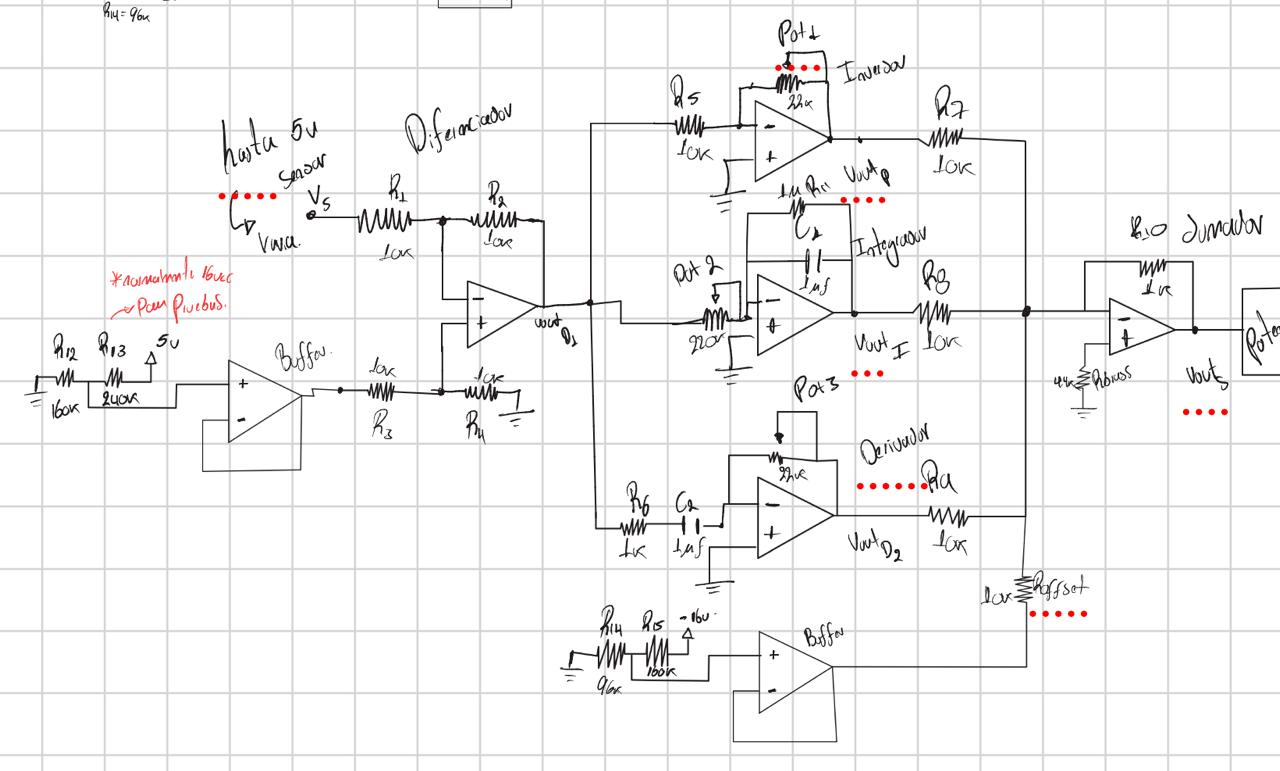
\includegraphics[width=1\linewidth]{circuito_manuscrito.jpeg}}{Esquemático a mano del controlador PID completo(puede verlo mas grande en los anexos).}

\IMG{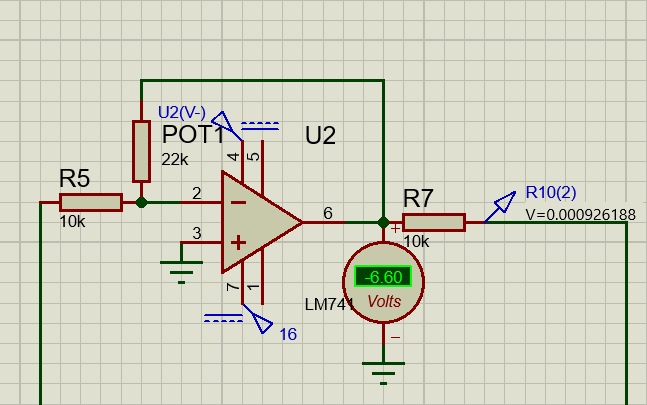
\includegraphics[width=1\linewidth]{proteus_inversor.png}}{Esquemático en Proteus inversor.}

\IMG{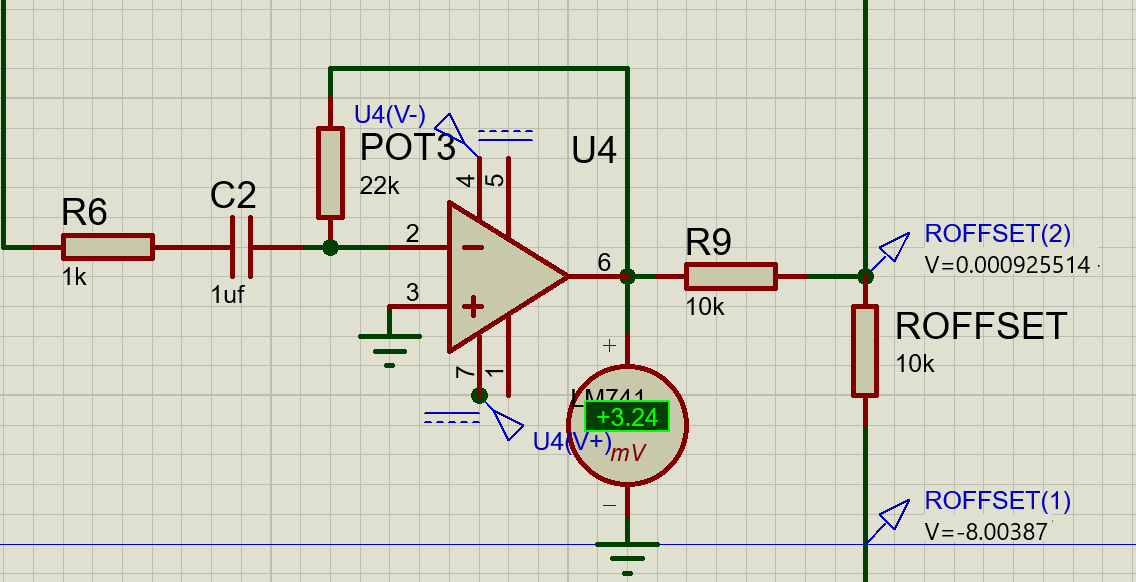
\includegraphics[width=1\linewidth]{proteus_derivador.png}}{Esquemático en Proteus integrador.}

\IMG{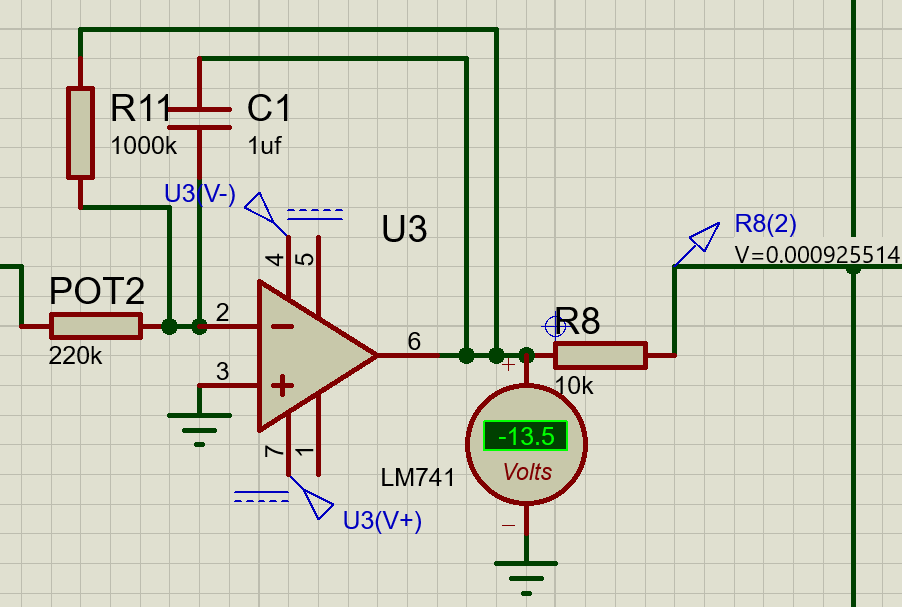
\includegraphics[width=0.9\linewidth]{proteus_integrador.png}}{Esquemático en Proteus derivador.}

\IMG{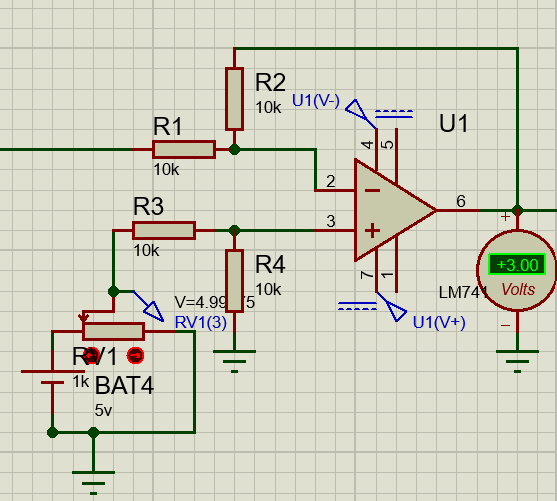
\includegraphics[width=0.9\linewidth]{proteus_diferenciador.png}}{Esquemático en Proteus diferenciador.}

\IMG{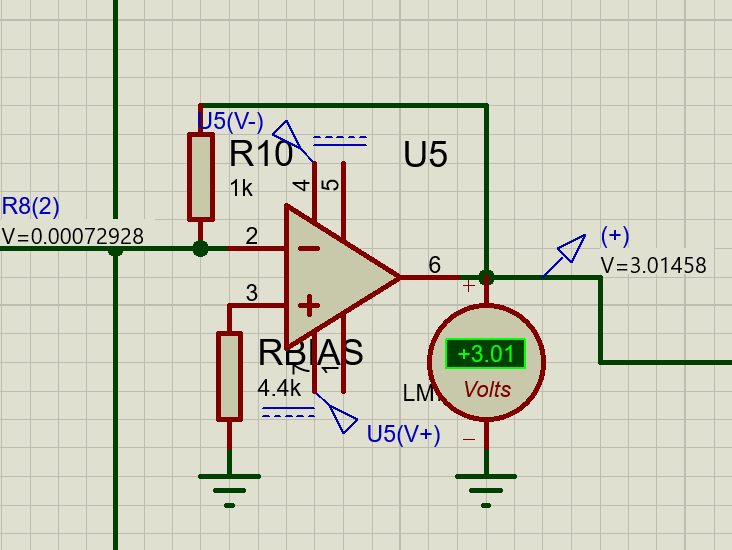
\includegraphics[width=0.9\linewidth]{proteus_sumador.png}}{Esquemático en Proteus sumador.}

\IMG{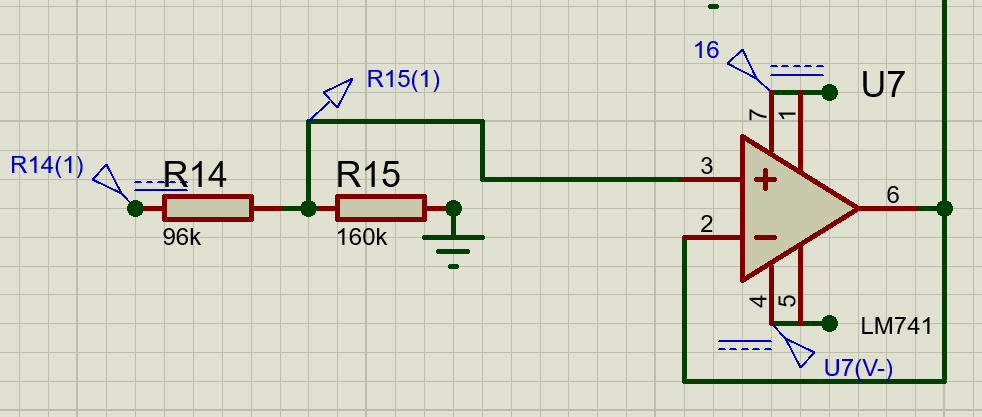
\includegraphics[width=0.9\linewidth]{proteus_buffer_voff.png}}{Esquemático en Proteus del controlador PID completo.}

\IMG{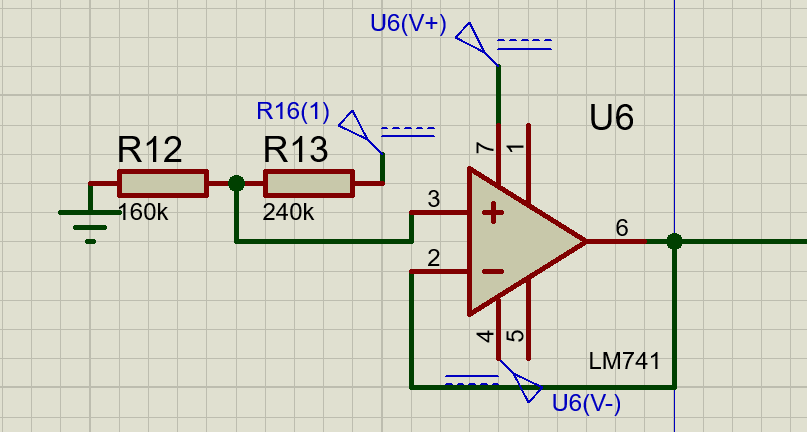
\includegraphics[width=0.9\linewidth]{proteus_buffer_vref.png}}{Esquemático en Proteus del controlador PID completo.}

\IMG{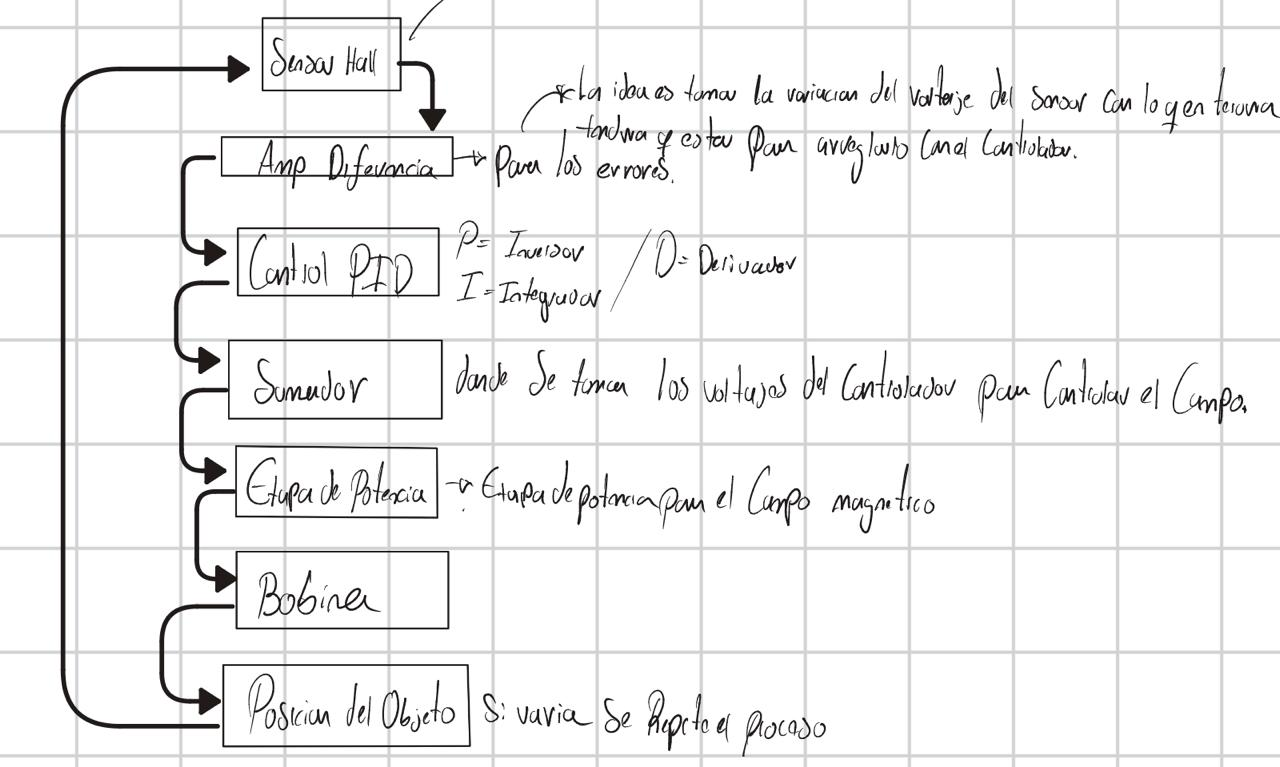
\includegraphics[width=0.9\linewidth]{diagrama_de_bloques.jpeg}}{Esquemático diagrama de bloques.}

\FOTO{pruebas/montaje_fisico.jpg}{Montaje físico del controlador PID: fuente de alimentación de $\pm$16~V, osciloscopio, multímetro y protoboard.}

\FOTO{pruebas/montaje_protoboard.jpg}{Circuito del controlador PID armado en protoboard con los siete amplificadores LM741.}

\FOTO{pruebas/medicion_diferenciador.jpg}{Toma de voltaje práctico con multímetro a la salida del diferenciador de error: $2.99$~V para el error máximo.}

\FloatBarrier
\subsection{Comparación de voltajes teóricos y prácticos}
La Tabla~\ref{tab:comparacion} resume, para cada etapa, el voltaje de entrada y de salida medido experimentalmente frente al valor teórico calculado, evaluado para error mínimo, medio y máximo.

\begin{table*}[t]
\centering
\caption{Comparación de voltajes teóricos y prácticos por etapa}
\label{tab:comparacion}
\small
\begin{tabular}{@{}l c c c c c c@{}}
\toprule
\multirow{2}{*}{\textbf{Etapa}} & \multicolumn{3}{c}{\textbf{Teórico (V)}} & \multicolumn{3}{c}{\textbf{Práctico (V)}} \\
\cmidrule(lr){2-4}\cmidrule(lr){5-7}
 & mín. & medio & máx. & mín. & medio & máx. \\
\midrule
Diferenciador & $-2$ & $0$ & $3$ & $-2.02$ & $0$ & $2.99$ \\
Proporcional (P) & $4.38$ & $-0.01$ & $-6.6$ & $4.46$ & $-0.15$ & $-6.6$ \\
Integral (I) & $9.14$ & $0.07$ & $-13.5$ & $6.22$ & $-0.32$ & $-13.22$ \\
Derivativo (D) & $-3.24\,\text{mV}$ & $-3.24\,\text{mV}$ & $-3.3\,\text{mV}$ & $3\,\text{mV}$ & $3\,\text{mV}$ & $172\,\text{mV}$ \\
Sumador & $-0.35$ & $1$ & $3.01$ & $-0.04$ & $1$ & $2.96$ \\
Divisor $V_{ref}$ & $2$ & $2$ & $2$ & $2$ & $2$ & $2$ \\
Divisor $V_{off}$ & $-10.1$ & $-10.1$ & $-10.1$ & $-10.21$ & $-10.21$ & $-10.21$ \\
\bottomrule
\end{tabular}
\end{table*}

\FloatBarrier
% =========================================================
\section{Lista de Componentes}
% =========================================================

\begin{table}[H]
\centering
\caption{Nomenclatura general del circuito}
\label{tab:nomenclatura}
\scriptsize
\begin{tabular}{@{}l p{5.7cm}@{}}
\toprule
\textbf{Ref.} & \textbf{Descripción} \\
\midrule
\multicolumn{2}{@{}l}{\textit{Diferenciador de error}} \\
$R_1$ & Entrada $V_{sensor}$ (rama inversora) \\
$R_{f1}$ & Realimentación del diferenciador \\
$R_3$ & Entrada $V_{ref}$ (rama no inversora) \\
$R_4$ & A GND (rama no inversora) \\
$U_1$ & LM741 --- Diferenciador de error \\
\midrule
\multicolumn{2}{@{}l}{\textit{Proporcional (P)}} \\
$R_5$ & Entrada fija ($10\,\text{k}\Omega$) \\
$Pot_1$ & Potenciómetro de realimentación, ajusta $K_p$ \\
$U_2$ & LM741 --- Etapa Proporcional \\
\midrule
\multicolumn{2}{@{}l}{\textit{Integral (I)}} \\
$Pot_2$ & Potenciómetro de entrada, ajusta $K_i$ ($R_i$) \\
$C_i$ & Capacitor de integración ($1\,\mu\text{F}$) \\
$R_6$ & Resistencia de fuga (anti-windup), en paralelo con $C_i$ \\
$U_3$ & LM741 --- Etapa Integral \\
\midrule
\multicolumn{2}{@{}l}{\textit{Derivativa (D)}} \\
$C_2$ & Capacitor de entrada ($1\,\mu\text{F}$) \\
$R_7$ & En serie con $C_2$, limita ganancia en alta frecuencia \\
$Pot_3$ & Potenciómetro de realimentación, ajusta $K_d$ \\
$U_4$ & LM741 --- Etapa Derivativa \\
\midrule
\multicolumn{2}{@{}l}{\textit{Sumador}} \\
$R_8$ & Entrada desde $V_P$ \\
$R_9$ & Entrada desde $V_I$ \\
$R_{10}$ & Entrada desde $V_D$ \\
$R_{11}$ & Entrada desde $V_{off}$ \\
$R_{12}$ & Realimentación del sumador \\
$U_5$ & LM741 --- Sumador \\
\midrule
\multicolumn{2}{@{}l}{\textit{Divisor + buffer de $V_{ref}$}} \\
$R_{13}$ & Divisor --- resistencia superior \\
$R_{14}$ & Divisor --- resistencia inferior \\
$U_6$ & LM741 --- Buffer no inversor \\
\midrule
\multicolumn{2}{@{}l}{\textit{Divisor + buffer de $V_{off}$}} \\
$R_{15}$ & Divisor --- resistencia superior \\
$R_{16}$ & Divisor --- resistencia inferior \\
$Pot_4$ & Ajuste fino del offset \\
$U_7$ & LM741 --- Buffer no inversor \\
\bottomrule
\end{tabular}
\end{table}

\begin{table*}[t]
\centering
\caption{Valores teóricos y finales ajustados}
\label{tab:valores}
\small
\begin{tabular}{@{}l c c l@{}}
\toprule
\textbf{Ref.} & \textbf{Teórico} & \textbf{Final (ajustado)} & \textbf{Obs.} \\
\midrule
$R_1$ & $10\,\text{k}\Omega$ & $10\,\text{k}\Omega$ & \\
$R_2$ & $10\,\text{k}\Omega$ & $10\,\text{k}\Omega$ & \\
$R_3$ & $10\,\text{k}\Omega$ & $10\,\text{k}\Omega$ & \\
$R_4$ & $10\,\text{k}\Omega$ & $10\,\text{k}\Omega$ & \\
$R_5$ & $10\,\text{k}\Omega$ & $10\,\text{k}\Omega$ & \\
$Pot_1$ & $33\,\text{k}\Omega$ & $22\,\text{k}\Omega$ & $K_p=2.2$ \\
$Pot_2$ & $12.5\,\text{k}\Omega$ & $220\,\text{k}\Omega$ & $K_i$ (ajustado) \\
$C_i\,(C_1)$ & $1\,\mu\text{F}$ & $1\,\mu\text{F}$ & \\
$R_6$ & $1\,\text{k}\Omega$ & $1\,\text{k}\Omega$ & \\
$C_2$ & $1\,\mu\text{F}$ & $1\,\mu\text{F}$ & \\
$R_7$ & $10\,\text{k}\Omega$ & $10\,\text{k}\Omega$ & \\
$Pot_3$ & $22\,\text{k}\Omega$ & $22\,\text{k}\Omega$ & $K_d=22$ \\
$R_8$ & $10\,\text{k}\Omega$ & $10\,\text{k}\Omega$ & Entrada $V_P$ (sumador) \\
$R_9$ & $10\,\text{k}\Omega$ & $10\,\text{k}\Omega$ & Entrada $V_I$ (sumador) \\
$R_{10}$ & $10\,\text{k}\Omega$ & $1\,\text{k}\Omega$ & Entrada $V_D$ (sumador) \\
$R_{11}$ & $1\,\text{M}\Omega$ & $1\,\text{M}\Omega$ & $K_{i,max}=4.5$ (fuga/anti-windup) \\
$R_{12}$ & $160\,\text{k}\Omega$ & $160\,\text{k}\Omega$ & Divisor $V_{ref}$ (fija) \\
$R_{13}$ & $240\,\text{k}\Omega$ & $240\,\text{k}\Omega$ & Divisor $V_{ref}$ ($V_{CC}=5\,$V) \\
$R_{14}$ & $96\,\text{k}\Omega$ & \textit{falta medir} & Divisor $V_{off}$ (calculada) \\
$R_{15}$ & $160\,\text{k}\Omega$ & $160\,\text{k}\Omega$ & Divisor $V_{off}$ (fija) \\
$R_{offset}$ & $10\,\text{k}\Omega$ & $10\,\text{k}\Omega$ & Entrada $V_{off}$ (sumador) \\
\bottomrule
\end{tabular}
\end{table*}

\FloatBarrier
% =========================================================
\section{Conclusiones}
% =========================================================

\subsection{Sobre la arquitectura de control}
El controlador PID en configuración paralela permitió cubrir, con un solo circuito, las tres necesidades dinámicas del sistema: corrección proporcional al error instantáneo (P), eliminación del error de estado estable mediante acumulación del historial reciente de error (I), y amortiguamiento ante transitorios rápidos (D). La conexión en paralelo, y no en cascada, fue indispensable para ajustar $K_p$, $K_i$ y $K_d$ de forma independiente.

\subsection{Sobre las correcciones de diseño}
La resistencia de anti-windup del integrador debe conectarse en paralelo con el capacitor de integración, nunca en serie: una conexión en serie deja la rama de realimentación en circuito abierto en continua y el amplificador opera prácticamente en lazo abierto. La ganancia en continua del integrador debe guardar una proporción razonable frente a $K_p$, ya que una ganancia DC excesiva provoca saturación ante errores muy por debajo del rango real de operación. Un divisor de voltaje resistivo solo entrega el voltaje calculado cuando la etapa que lo carga presenta una impedancia de entrada considerablemente mayor que las resistencias del propio divisor; este efecto de carga se resolvió con un buffer no inversor en cada divisor. El rango de salida (1~V a 3~V) se logró mediante dos ajustes independientes y secuenciales: la ganancia del sumador, que define el ancho del rango, y el offset, que define su punto de partida.

\subsection{Sobre el comportamiento observado}
La etapa derivativa opera en el rango de milivoltios la mayor parte del tiempo, alcanzando el rango de voltios solo durante transitorios rápidos del error, dado que la dinámica mecánica del sistema es comparativamente lenta frente a la respuesta eléctrica del circuito. El offset de entrada de los amplificadores LM741 (1 a 6~mV típico) resulta despreciable frente a las señales de voltios manejadas por P y el sumador, pero se vuelve relevante al amplificarse por la ganancia en continua del integrador.

\subsection{Efecto de carga en los divisores resistivos}
Se verificó experimentalmente que los divisores resistivos diseñados para $V_{ref}$ y $V_{off}$ no entregaban el voltaje teórico calculado al conectarse a la etapa siguiente: el voltaje medido variaba y disminuía bajo carga. Este comportamiento corresponde al efecto de carga de un divisor resistivo, que solo entrega el voltaje calculado con precisión cuando la resistencia de la etapa siguiente es considerablemente mayor que las resistencias del propio divisor. La solución aplicada fue intercalar un amplificador operacional en configuración de seguidor de voltaje (buffer no inversor, ganancia unitaria) entre cada divisor y la etapa que utiliza esa referencia, aprovechando la alta impedancia de entrada del operacional para no cargar el divisor.

Nota (Algunos cambios practicos e explicaciones mas profundas se encuetran en el apartado IV)
% =========================================================
\begin{thebibliography}{00}
\bibitem{earnshaw1842} S. Earnshaw, ``On the nature of the molecular forces which regulate the constitution of the luminiferous ether,'' \emph{Transactions of the Cambridge Philosophical Society}, vol. 7, pp. 97--112, 1842.
\bibitem{berkelman} P. Berkelman and S. Kang, ``Optimization of the Four Coil Configuration for Single Magnet Levitation from Below,'' University of Hawaii at M\=anoa, Honolulu, HI, USA.
\bibitem{lm741} Texas Instruments, ``LM741 Operational Amplifier,'' datasheet.
\bibitem{ss495a} Honeywell, ``SS490 Series / SS495A Linear Hall-Effect Sensor,'' datasheet.
\bibitem{tip122} STMicroelectronics, ``TIP122 --- NPN Darlington Power Transistor,'' datasheet.
\bibitem{ogata} K. Ogata, \emph{Modern Control Engineering}, 5th ed. Upper Saddle River, NJ, USA: Prentice Hall, 2010.
\end{thebibliography}

% =========================================================
\appendix[Índice de Cálculos a Mano]
% =========================================================

La Tabla~\ref{tab:anexo} indexa las imágenes de los cálculos realizados a mano durante el desarrollo del proyecto, referenciando la etapa a la que corresponde cada una.

\begin{table}[H]
\centering
\caption{Índice de anexos de imágenes}
\label{tab:anexo}
\scriptsize
\resizebox{\linewidth}{!}{%
\begin{tabular}{@{}c p{4.2cm} l@{}}
\toprule
\textbf{N.\textdegree} & \textbf{Descripción} & \textbf{Etapa} \\
\midrule
1 & Circuito completo simulado en Proteus & Montaje \\
2 & Circuito armado físicamente (fotografía) & Montaje \\
3--4 & Derivación del diferenciador (amplificador diferencial) & Diferenciador \\
5--6 & Derivación de la etapa inversora / Proporcional & P \\
7--8 & Derivación del integrador, Laplace y anti-windup & I \\
9--10 & Derivación del derivador y filtro en alta frecuencia & D \\
11 & Derivación del sumador y $R_{bias}$ & Sumador \\
12 & Cálculos de los divisores de $V_{ref}$ y $V_{off}$ & Offset/Ref. \\
13 & Ajuste de ganancias del sumador por saturación y offset & Sumador \\
14--19 & Tomas de voltajes prácticos por etapa (6 imágenes) & Resultados \\
\bottomrule
\end{tabular}%
}
\end{table}

\IMGPAGE{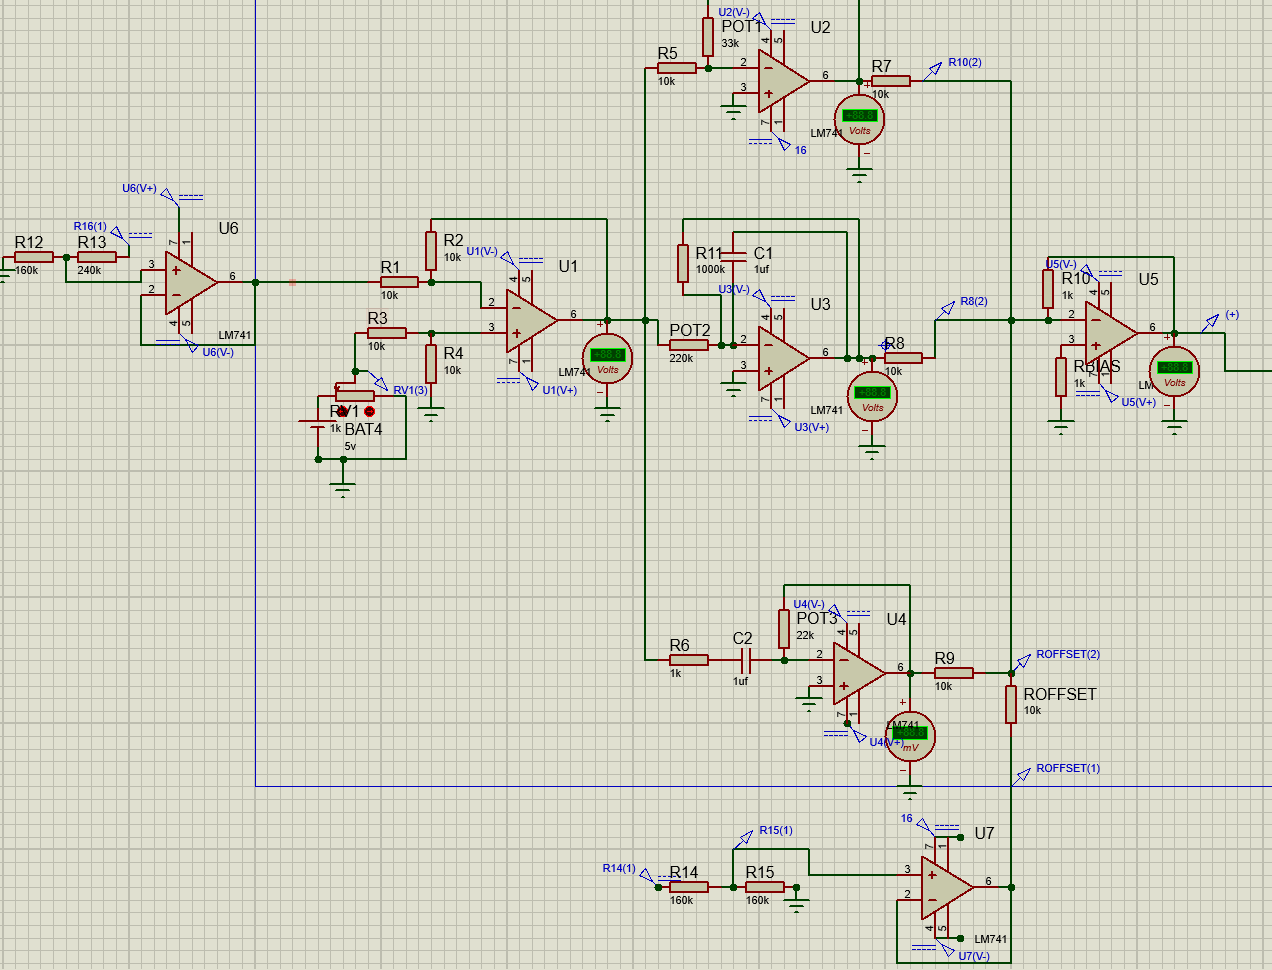
\includegraphics[width=1\linewidth,height=1\textheight,keepaspectratio]{proteus_circuito_completo.png}}{Esquematico de proteous.}

\IMGPAGE{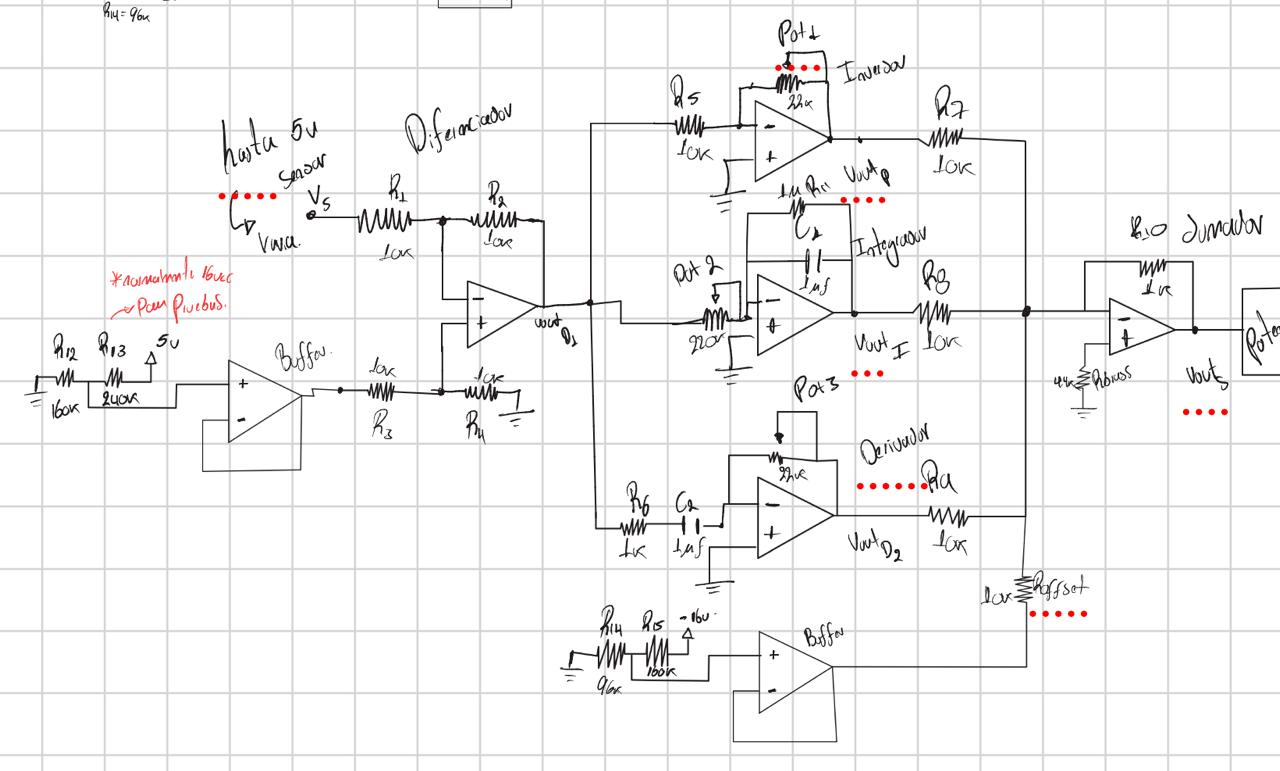
\includegraphics[width=1\linewidth,height=1\textheight,keepaspectratio]{circuito_manuscrito.jpeg}}{Esquematico hecho a mano.}

\IMGPAGE{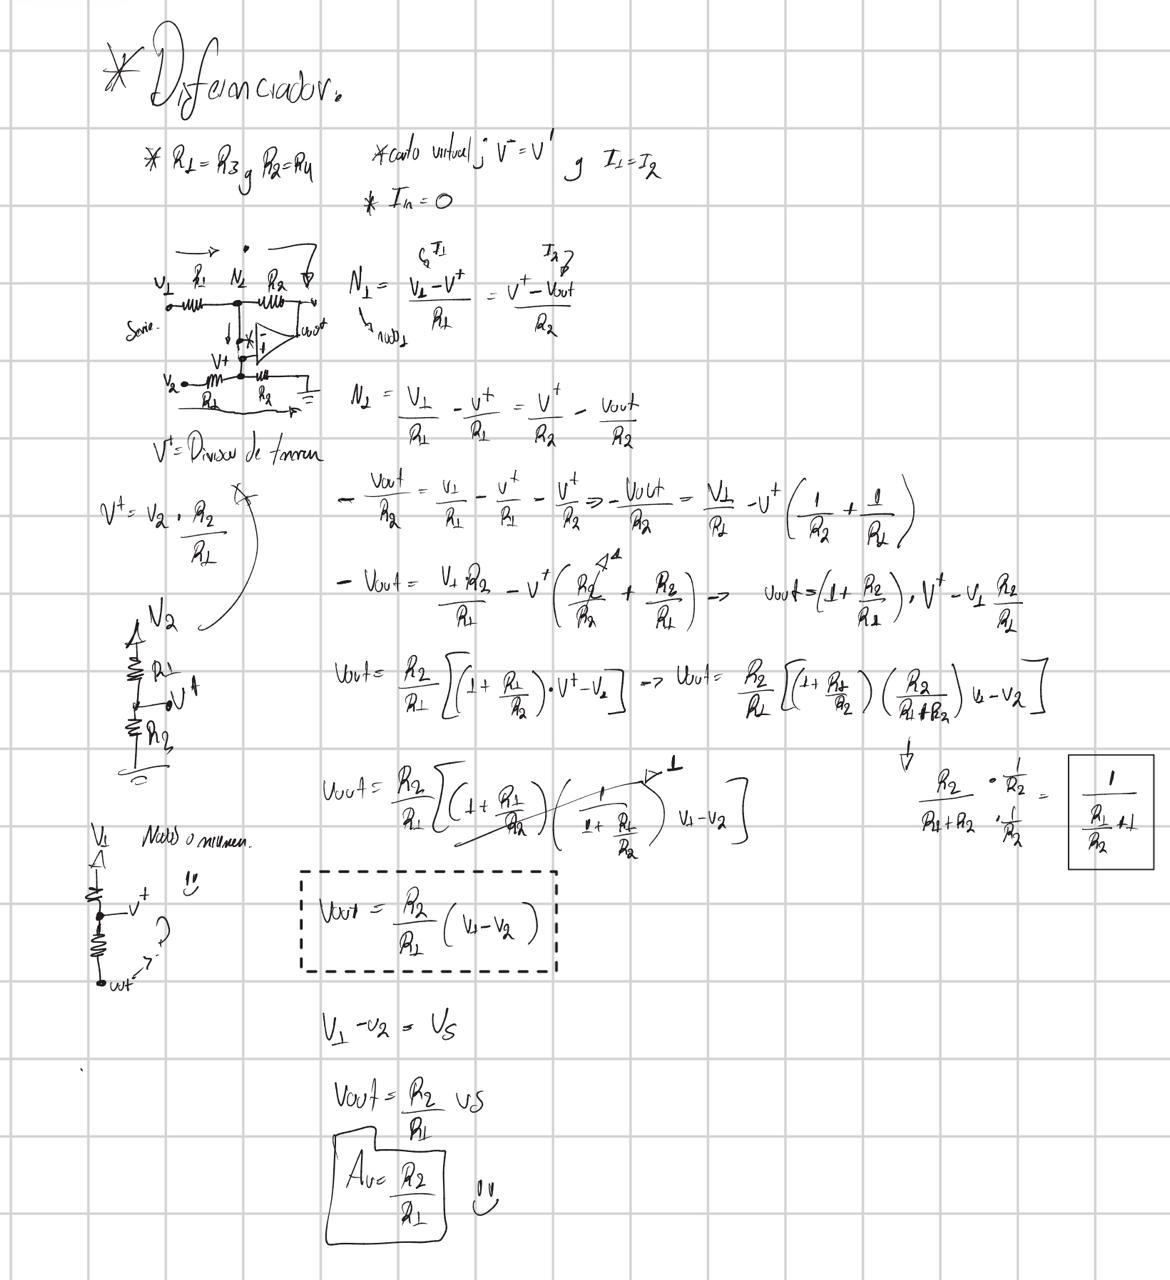
\includegraphics[width=1\linewidth,height=0.85\textheight,keepaspectratio]{calculo_diferenciador_1.jpeg}}{Cálculos diferenciador (1).}
\IMGPAGE{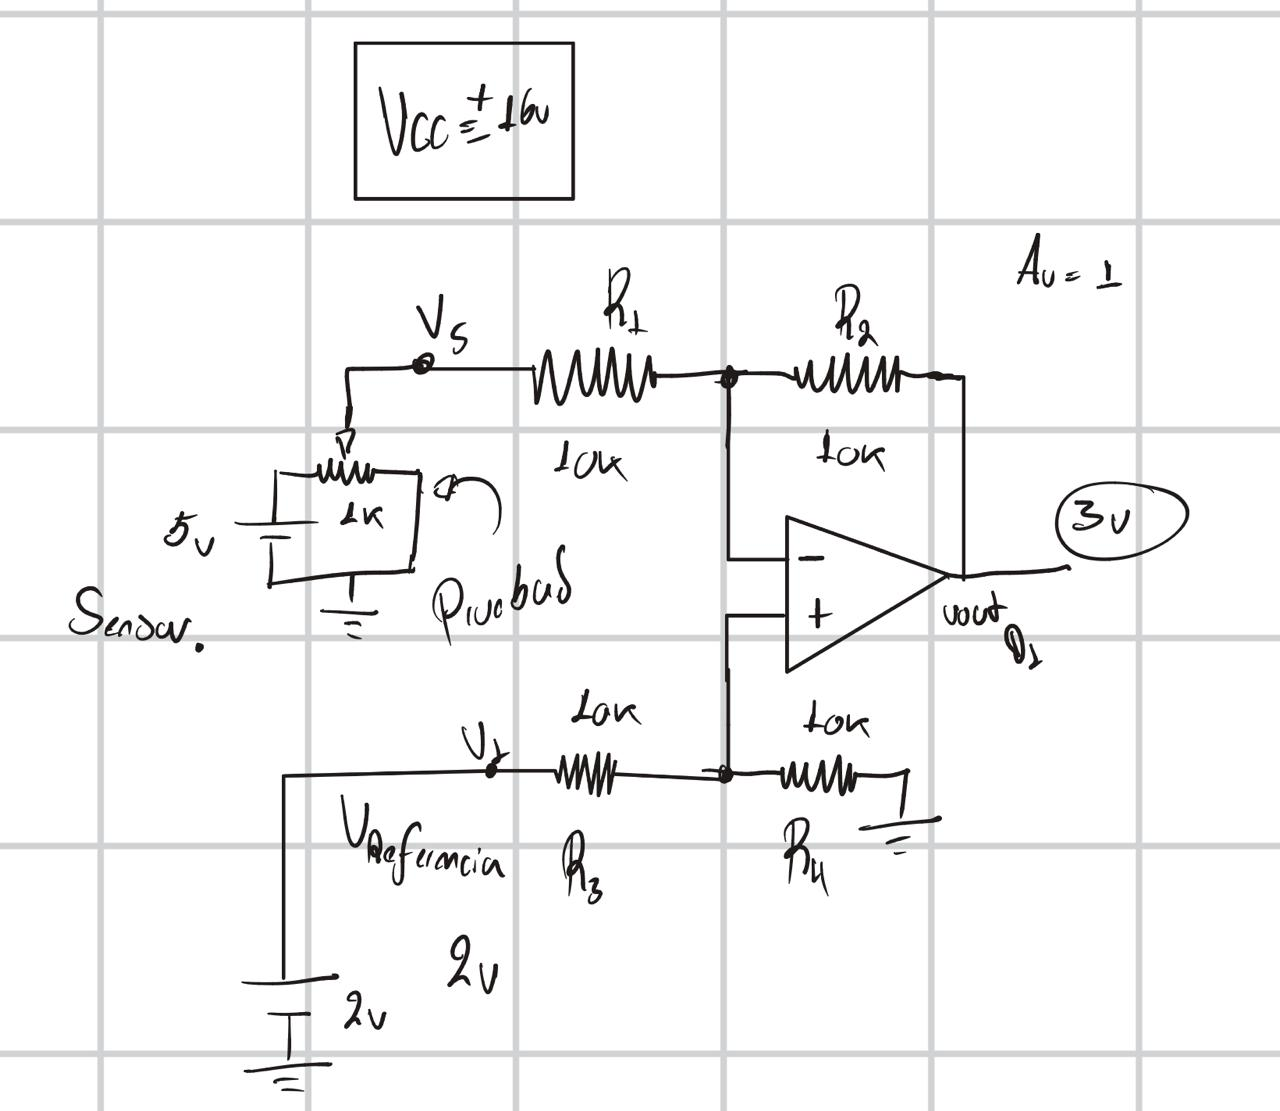
\includegraphics[width=1\linewidth,height=0.85\textheight,keepaspectratio]{calculo_diferenciador_2.jpeg}}{Cálculos diferenciador (2).}

\IMGPAGE{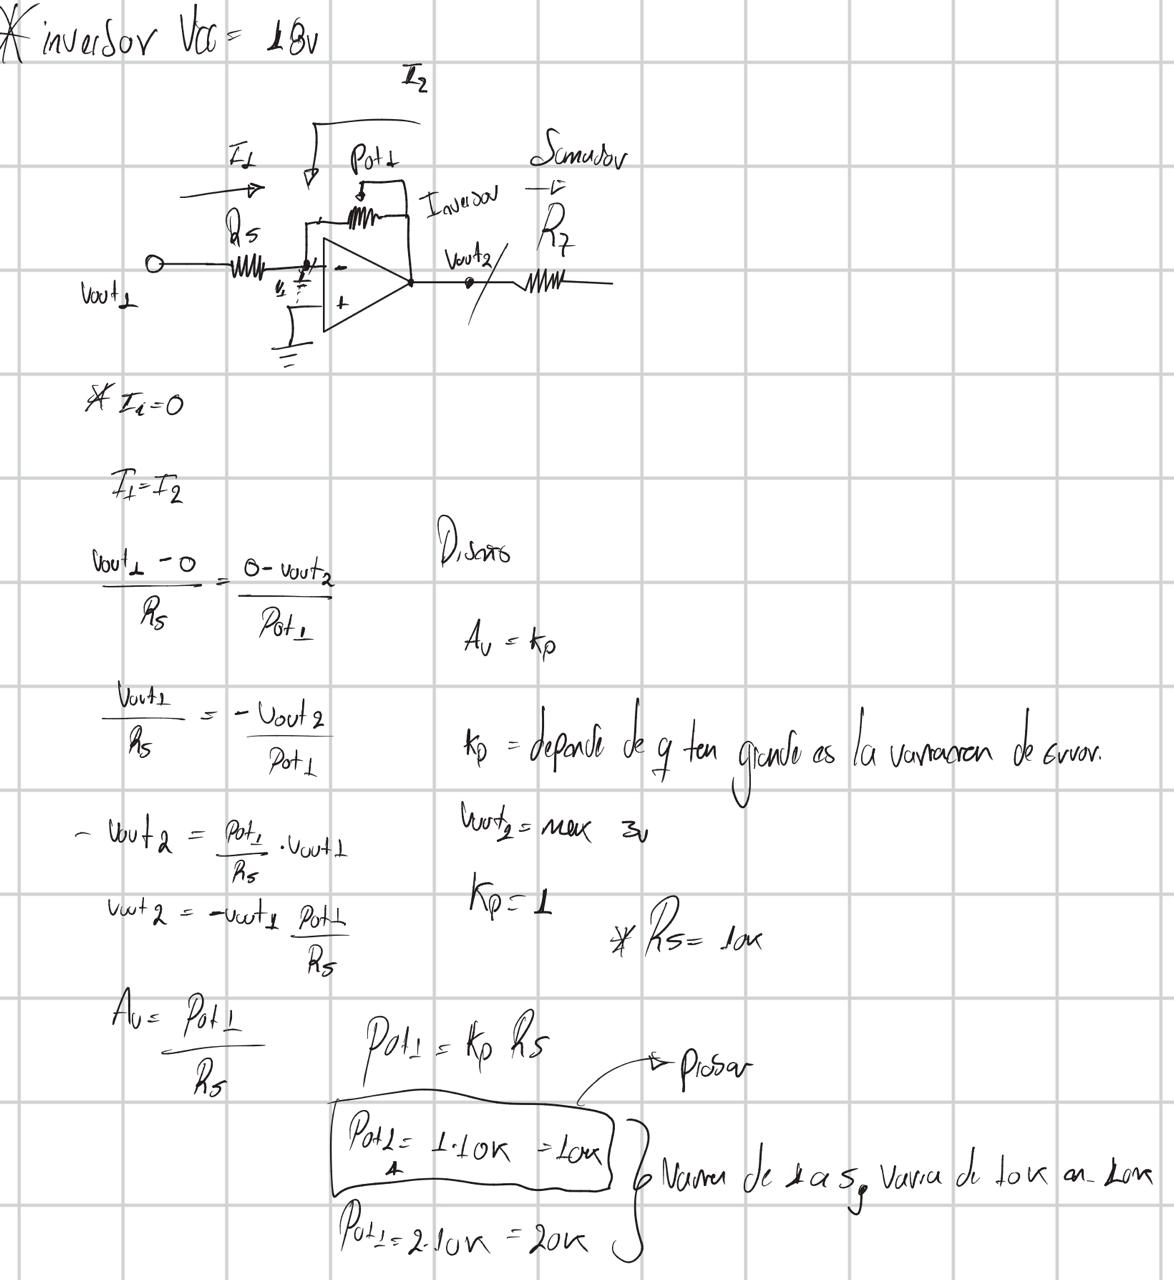
\includegraphics[width=0.92\linewidth,height=0.85\textheight,keepaspectratio]{calculo_inversor_1.jpeg}}{Cálculos inversor (1).}
\IMGPAGE{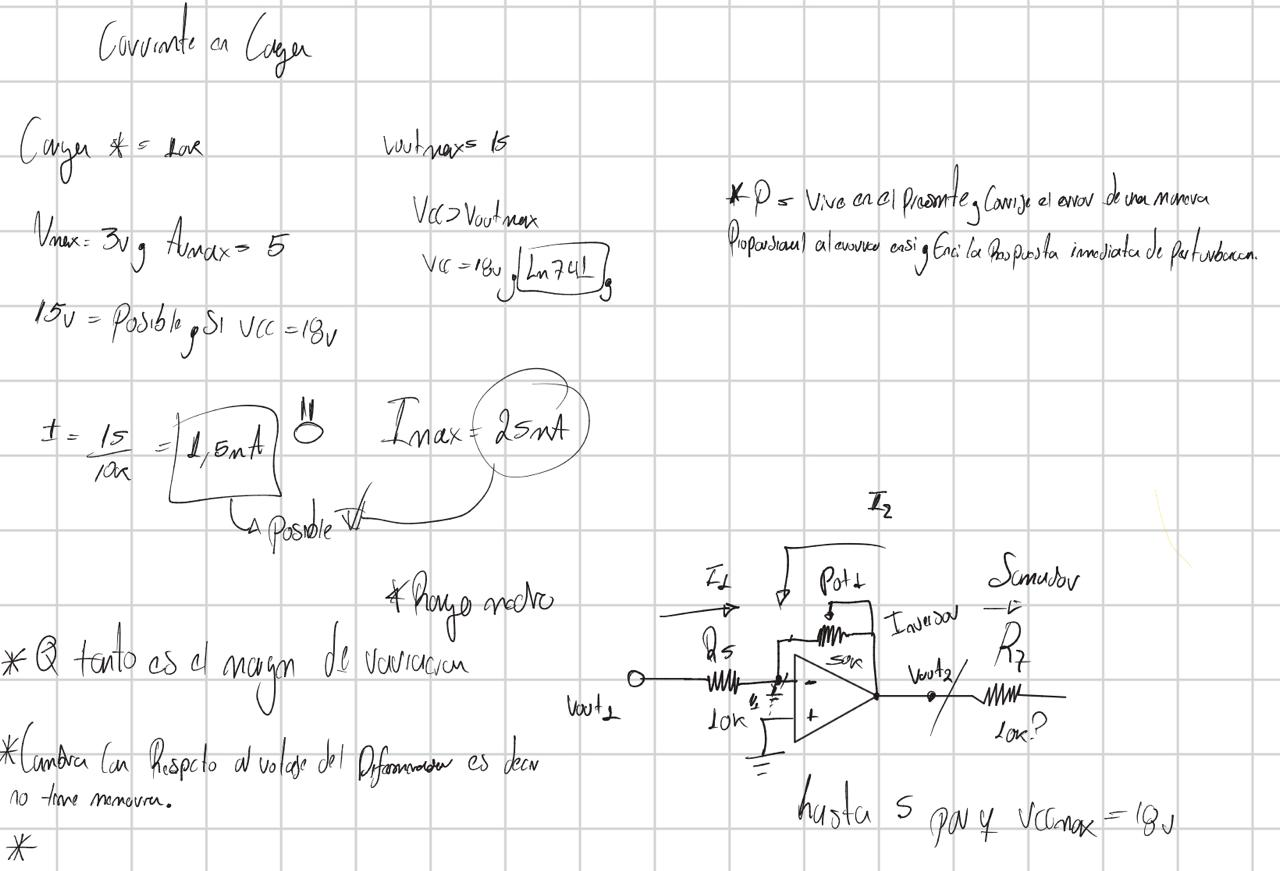
\includegraphics[width=0.92\linewidth,height=0.85\textheight,keepaspectratio]{calculo_inversor_2.jpeg}}{Cálculos inversor (2).}

\IMGPAGE{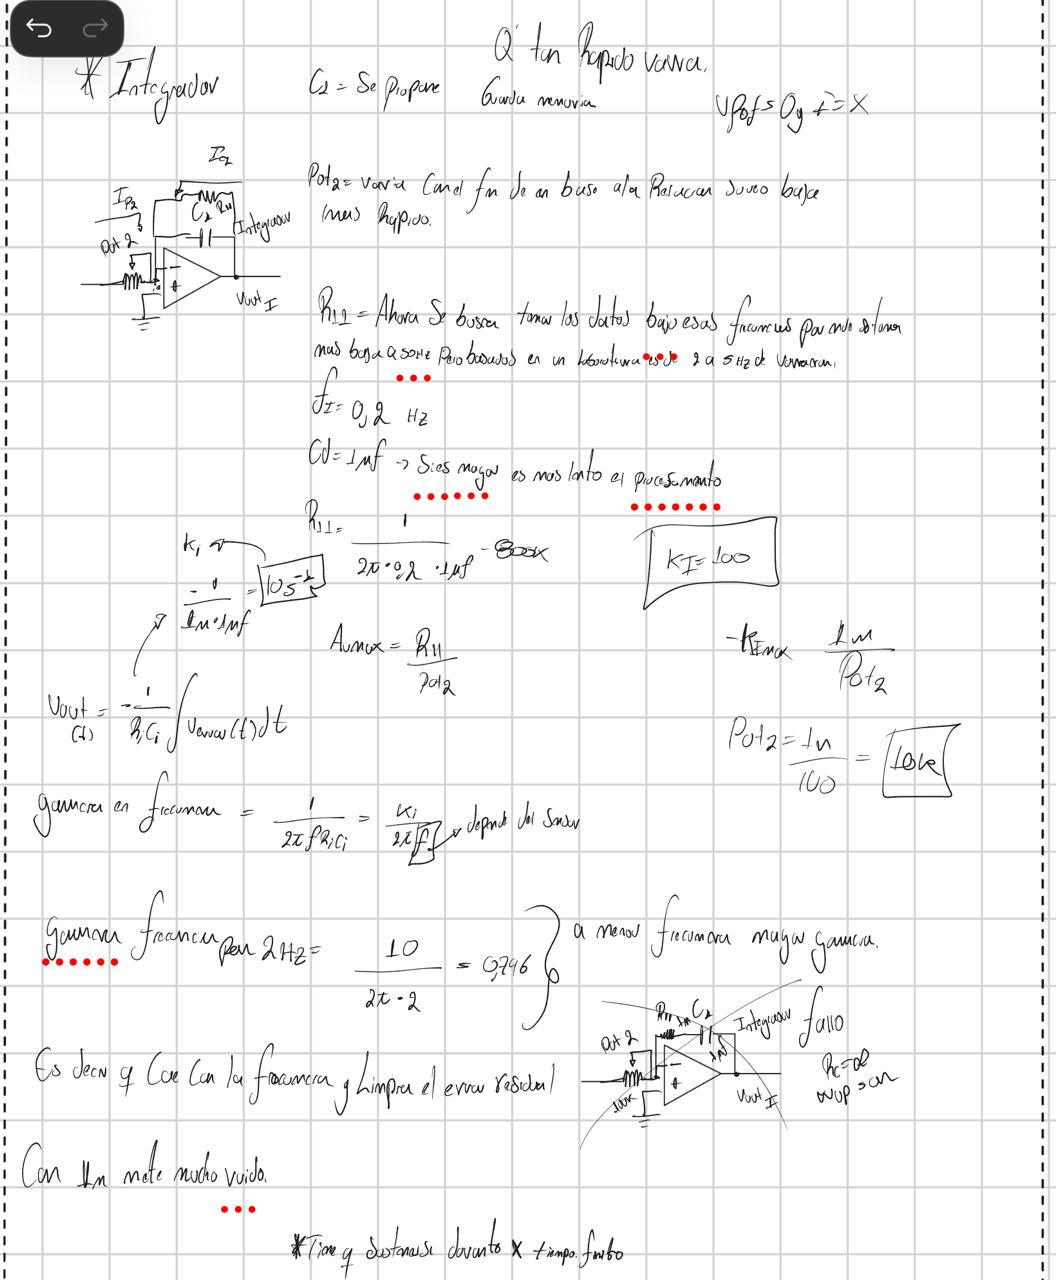
\includegraphics[width=0.92\linewidth,height=0.85\textheight,keepaspectratio]{calculo_integrador_1.jpeg}}{Cálculos integrador (1).}
\IMGPAGE{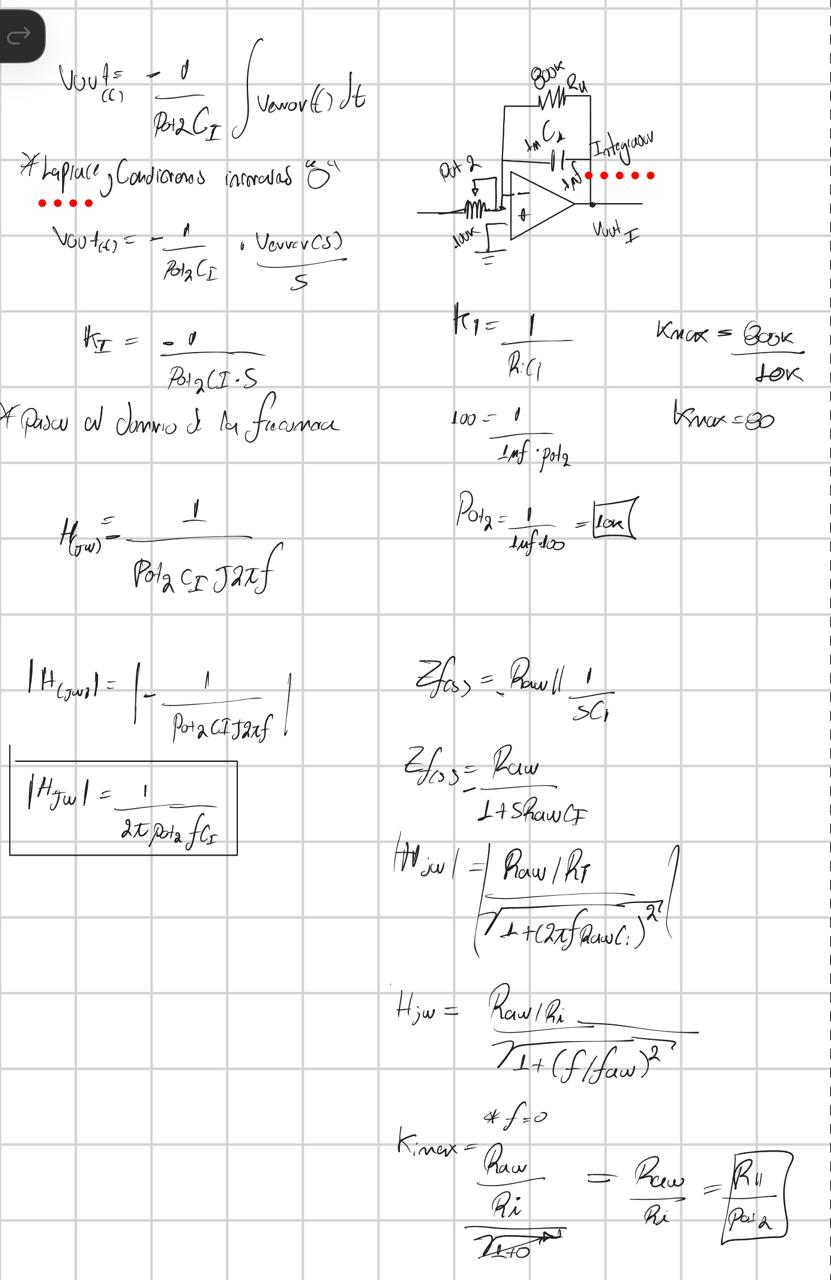
\includegraphics[width=0.92\linewidth,height=0.85\textheight,keepaspectratio]{calculo_integrador_2.jpeg}}{Cálculos integrador (2).}

\IMGPAGE{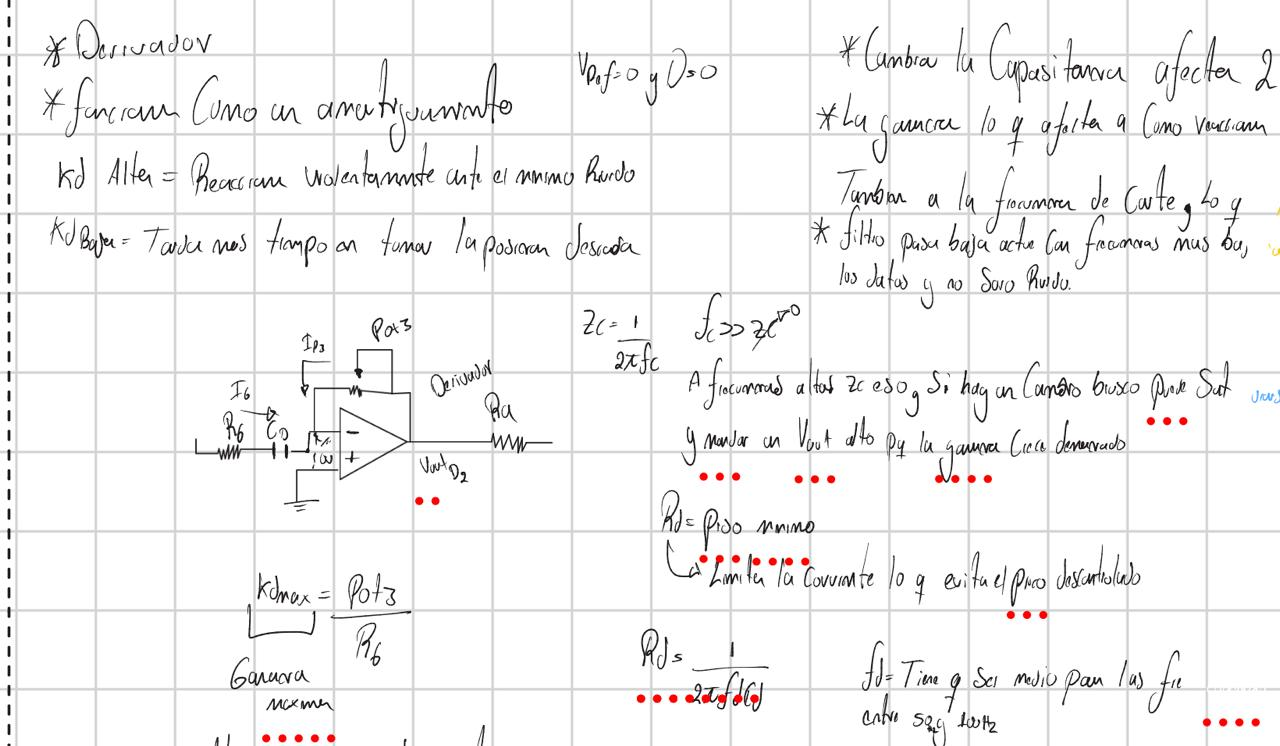
\includegraphics[width=0.92\linewidth,height=0.85\textheight,keepaspectratio]{calculo_derivador_1.jpeg}}{Cálculos Derivador (1).}
\IMGPAGE{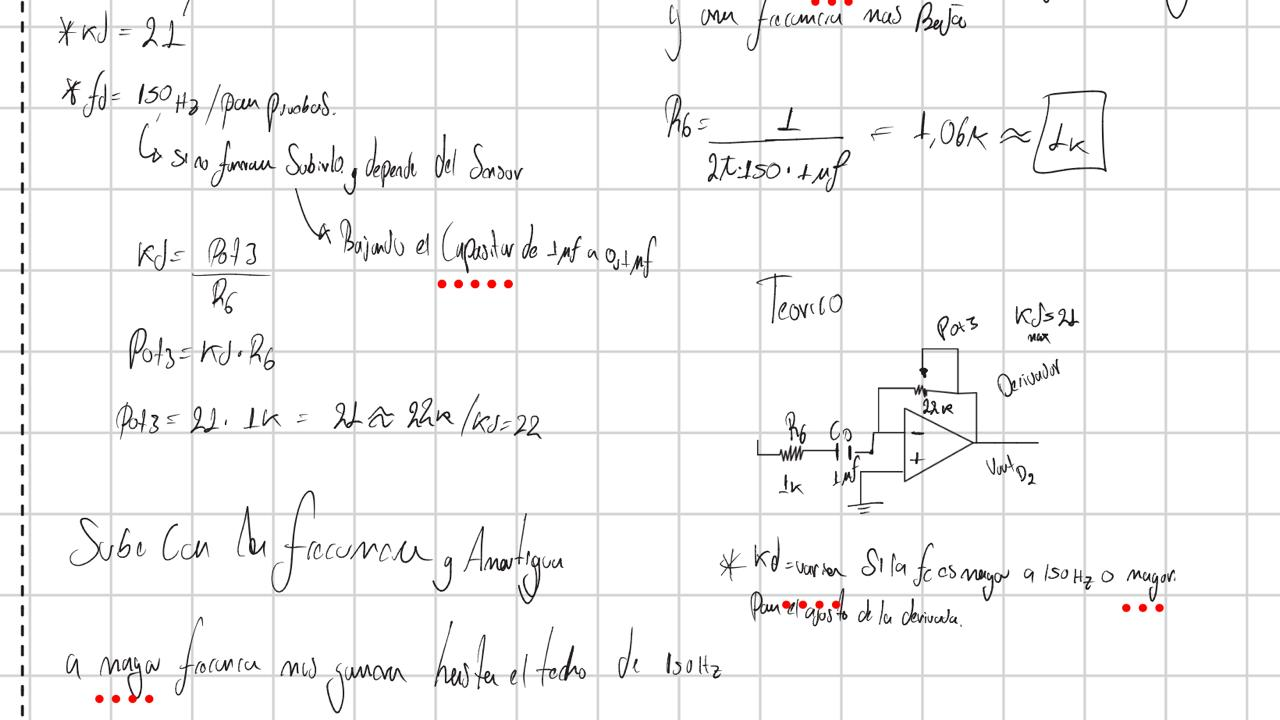
\includegraphics[width=1\linewidth,height=1\textheight,keepaspectratio]{calculo_derivador_2.jpeg}}{Cálculos Derivador (2).}

\IMGPAGE{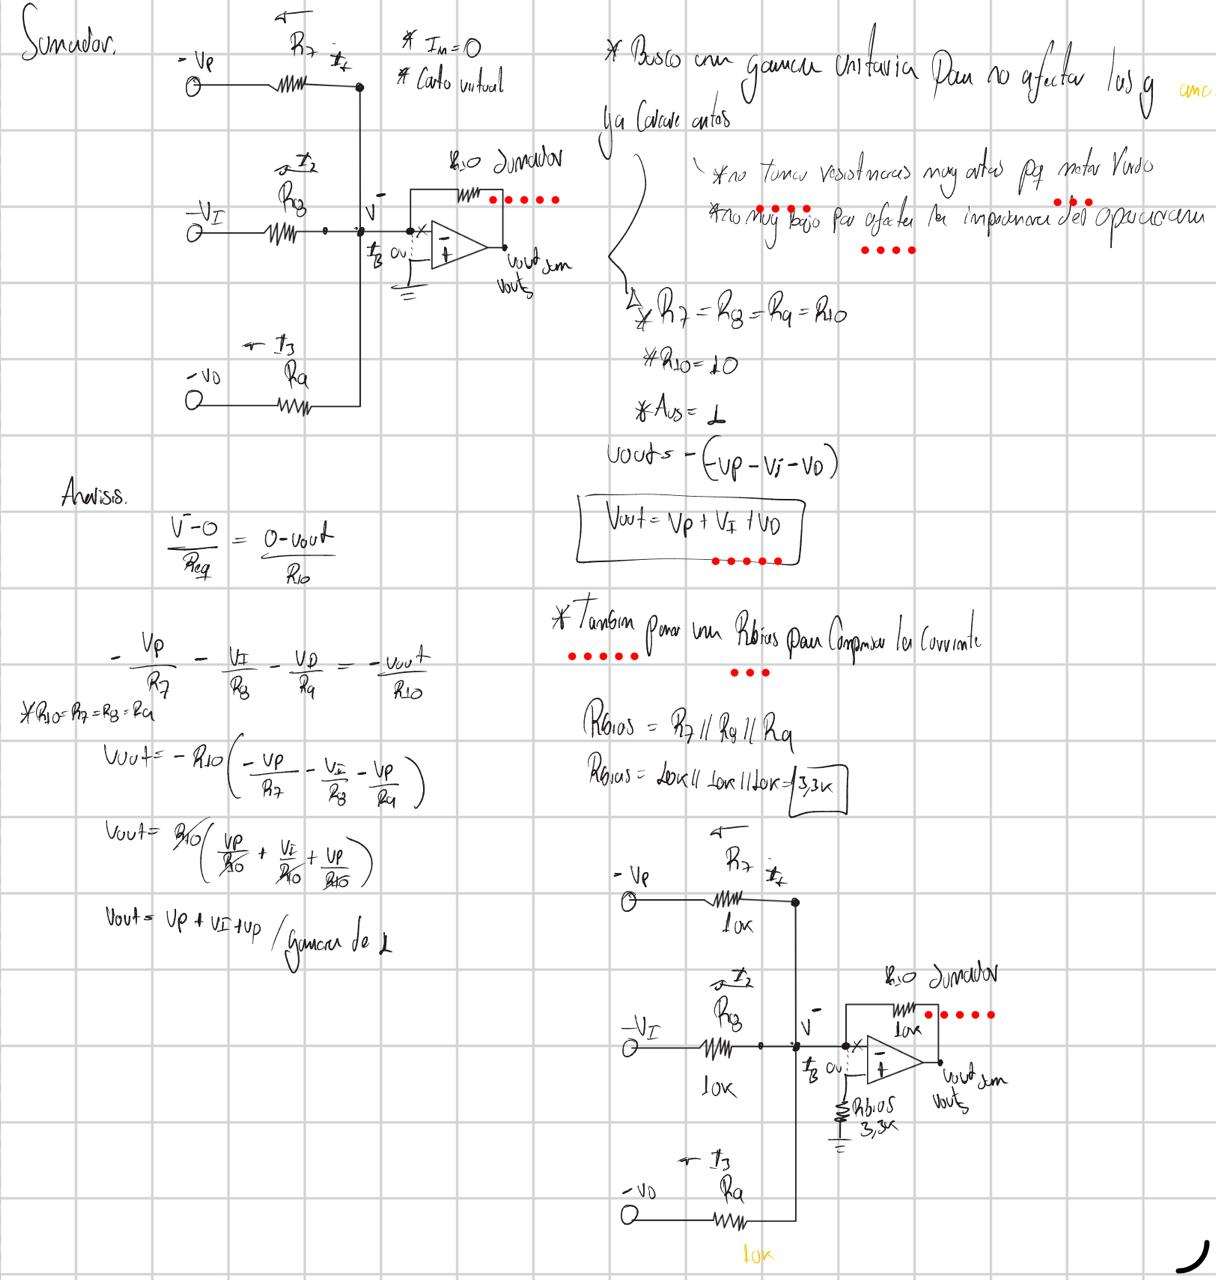
\includegraphics[width=1\linewidth,height=1\textheight,keepaspectratio]{calculo_sumador.jpeg}}{Cálculos Sumador.}
\IMGPAGE{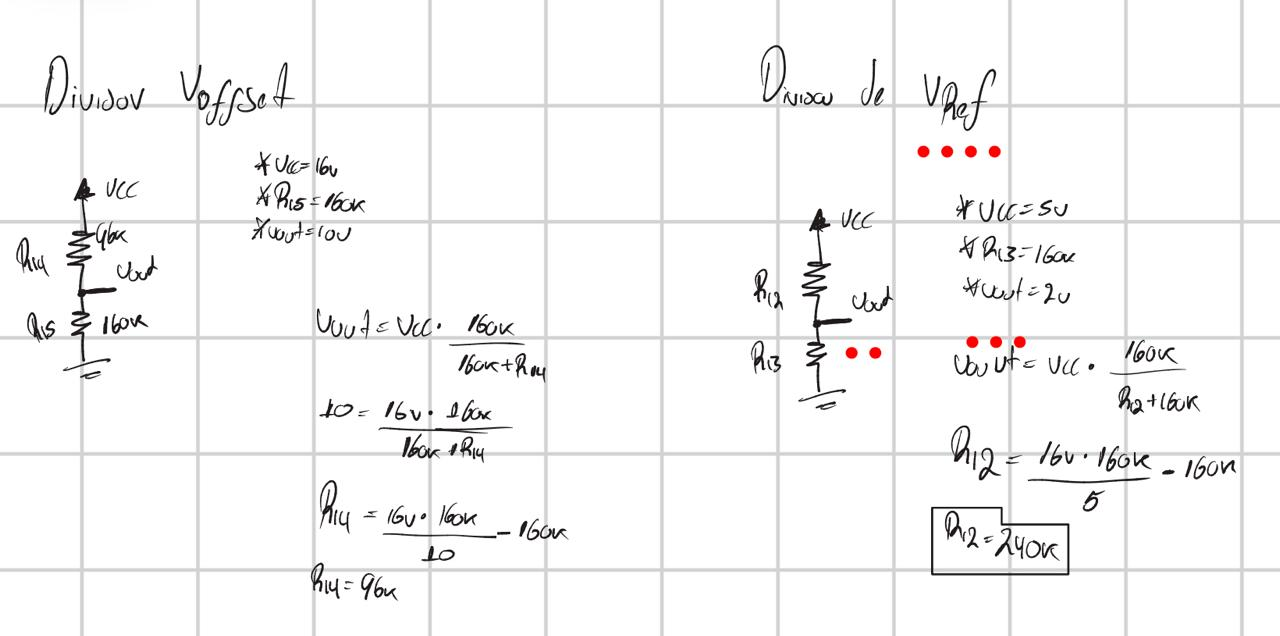
\includegraphics[width=0.92\linewidth,height=0.85\textheight,keepaspectratio]{calculo_divisores.jpeg}}{Cálculos divisor Voffset y Vref.}

\IMGPAGE{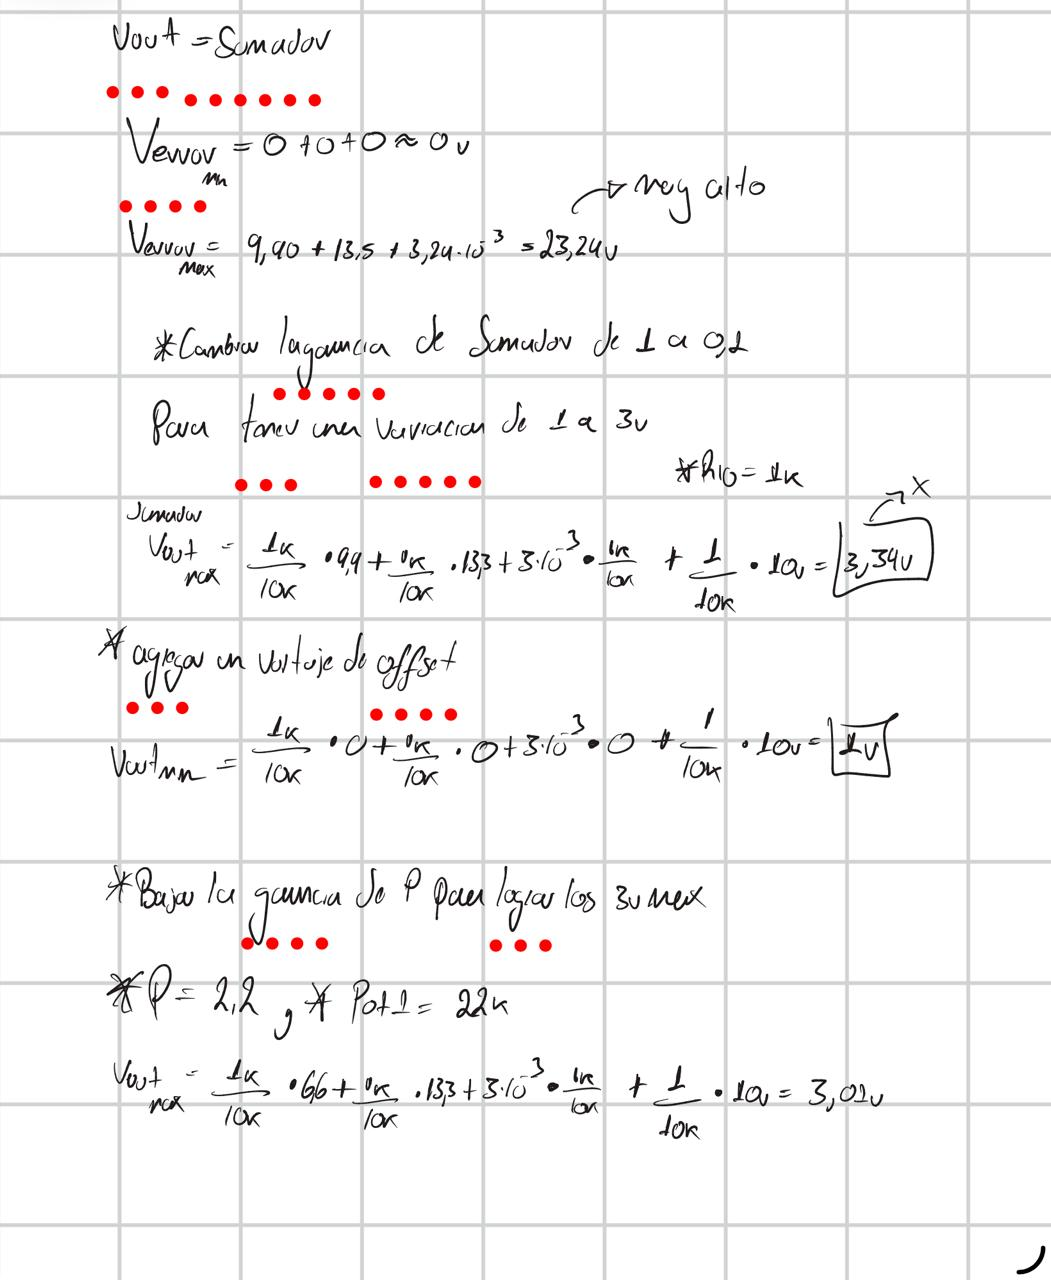
\includegraphics[width=1\linewidth,height=1\textheight,keepaspectratio]{calculo_sumador_ajuste_final.jpeg}}{Cambios finales al sumador.}

% =========================================================
% PLANTILLA: copia y pega este bloque una vez por cada imagen
% adicional (cálculos 10 a 20). Para una foto real, reemplaza
% el primer argumento por:
%   \includegraphics[width=0.92\linewidth,height=0.85\textheight,keepaspectratio]{ruta_de_tu_imagen.jpg}
% =========================================================
% \IMGPAGE{Descripción del cálculo manuscrito}{Cálculos manuscritos --- Descripción corta (N.).}

\end{document}